\باب{کولمب کا قانون}\شناخت{باب_کولمب_قانون}
\حصہ{قوت کشش یا دفع}
نیوٹن کے \اصطلاح{کائناتی تجاذب کے قانون}\فرہنگ{تجاذب}\حاشیہب{Law of Universal Gravitation} سے آپ بخوبی واقف ہوں گے۔\اصطلاح{کولمب کا قانون}\فرہنگ{کولمب کا قانون}\حاشیہب{Coulomb's law} اس سے قریبی مشابہت رکھتا ہے۔کائناتی تجاذب کے قانون کو مساوات \حوالہ{مساوات_کولوم_کشش_ثقل} میں پیش کیا گیا ہے۔
\begin{align}\label{مساوات_کولوم_کشش_ثقل}
F&=G \frac{M_1 M_2}{R^2}
\end{align}
یہ مساوات کمیت \عددیء{M_1} اور کمیت \عددیء{M_2} کے مابین قوت کشش \عددیء{F} دیتا ہے جہاں ایک کمیت کے مرکز سے دوسری کمیت کے مرکز تک کا فاصلہ \عددیء{R} ہے۔قوت کشش دونوں کمیت کے حاصل ضرب کے  راست متناسب اور ان کے مرکزوں کے درمیانی فاصلے  کے مربع کے بالعکس متناسب ہوتی ہے۔دونوں کمیتوں پر قوت کشش کی مقدار برابر ہوتی ہے اور یہ قوت دونوں کمیتوں کے  مرکزوں پر کھینچی لکیر پر عمل درآمد ہوتی ہے۔\عددیء{M_1} پر قوت کشش کی سمت \عددیء{M_1} کے مرکز سے \عددیء{M_2} کے مرکز کی جانب کو ہوتا ہے جبکہ \عددیء{M_2} پر قوت کشش کی سمت \عددیء{M_2} کے مرکز سے \عددیء{M_1} کے مرکز کی جانب کو ہوتا ہے۔تناسب کے جزو مستقل کو \عددیء{G} لکھا اور \اصطلاح{تجاذبی مستقل}\فرہنگ{تجاذبی مستقل}\حاشیہب{gravitational constant}\فرہنگ{gravitational constant} پکارا جاتا ہے جس کی قیمت تقریباً \عددیء{\SI{6.674e-11}{\meter \cubed \per \kilo \gram \per \second \squared}} کے برابر ہے۔کرہ ارض کے ثقلی میدان میں میکانی بار \عددی{m} کو اٹھانے کی خاطر \عددی{F=m g} قوت درکار ہوتی  ہے جہاں \عددی{g=\SI{9.8}{\meter\per\second\squared}} کے برابر ہے۔

کولمب کا قانون مساوات \حوالہ{مساوات_کولوم_کولمب_کشش_بار} میں بیان کیا گیا ہے۔یہ مساوات \اصطلاح{برقی بار}\فرہنگ{برقی بار}\حاشیہب{charge}\فرہنگ{charge} \عددیء{Q_1} اور برقی بار \عددیء{Q_2} کے مابین قوت کشش یا قوت دفع \عددیء{F} دیتا ہے جہاں ایک برقی بار کے مرکز سے دوسری برقی بار کے مرکز تک کا فاصلہ \عددیء{R} ہے۔ان برقی باروں کا حجم صفر تصور کیا جاتا ہے۔یوں اگر برقی بار کو گیند کی شکل کا تصور کیا جائے تو اس گیند کے رداس  کی لمبائی صفر ہو گی۔ایسے برقی بار کو \اصطلاح{نقطہ برقی بار}\فرہنگ{نقطہ برقی بار}\حاشیہب{point charge}\فرہنگ{point charge} کہا جاتا ہے۔برقی بار کو \اصطلاح{برق}\فرہنگ{برق} یا \اصطلاح{بار}\فرہنگ{بار} کہا جائے گا۔
\begin{align}\label{مساوات_کولوم_کولمب_کشش_بار}
F&=\frac{1}{4 \pi \epsilon_0}\frac{Q_1 Q_2}{ R^2}
\end{align}

قوت کشش یا دفع دونوں برقی باروں کے حاصل ضرب کے  راست متناسب  اور باہمی فاصلہ کے  مربع کے بالعکس متناسب ہوتی ہے۔دونوں برقی باروں پر قوت کی مقدار برابر ہوتی ہے اور یہ قوت دونوں برقی باروں سے گزرتی لکیر پر عمل درآمد ہوتی ہے۔دو مختلف اقسام کے برقی باروں کے مابین قوت کشش پائی جاتی ہے جبکہ دو یکساں برقی باروں کے مابین قوت دفع پائی جاتی ہے۔مساوات کے جزو مستقل کو \عددیء{\tfrac{1}{4 \pi \epsilon_0}} لکھا جاتا ہے جہاں \عددیء{\epsilon_0} خالی خلاء  کا \اصطلاح{برقی مستقل}\فرہنگ{برقی مستقل}\حاشیہب{permittivity}\فرہنگ{permittivity}\حاشیہب{electric constant}\فرہنگ{electric constant} ہے جس کی قیمت اٹل ہے۔خالی خلاء کے برقی مستقل کی قیمت
\begin{align}
\epsilon_0=\frac{1}{\mu_0 c^2}
\end{align}
ہے جہاں \عددیء{c} خالی خلاء میں روشنی کی رفتار اور \عددیء{\mu_0} خالی خلاء کی \اصطلاح{مقناطیسی مستقل}\فرہنگ{مقناطیسی مستقل}\حاشیہب{permeability}\فرہنگ{permeability} ہے۔یہ دونوں بھی اٹل مستقل ہیں جن کی قیمتیں
\begin{align}
c&=\SI{299792458}{\meter \per \second} \approx \SI{3e8}{\meter \per \second}\\
\mu_0&=\SI{4 \numpi e-7}{\henry \per \meter}
\end{align}
 ہیں۔یوں مقناطیسی مستقل  کی قیمت تقریباً
\begin{align}
\epsilon_0 =\num{8.854e-12} \overset{.}{=}\frac{1}{36 \pi} 10^{-9} \si{\farad \per \meter}
\end{align}
 کے برابر ہے۔اس کتاب میں \عددیء{\tfrac{1}{4 \pi \epsilon_0}} بار بار استعمال ہو گا جسے عموماً
\begin{align}\label{مساوات_کولمب_برقی_مستقل_قیمت_الف}
\frac{1}{4 \pi \epsilon_0} \overset{.}{=} 9 \times 10^9
\end{align}
لیا جائے گا۔\عددیء{\epsilon_0}  کی اکائی فیراڈ فی میٹر  \عددیء{\si{\farad \per \meter}} ہے  جس کی وضاحت جلد کر دی جائے گی۔

\ابتدا{مثال}
زمین کی سطح پر زمین اور ایک کلو گرام کمیت کے مابین \عددیء{\SI{9.8}{\newton}} کی قوت کشش پائی جاتی ہے۔زمین کا رداس \عددیء{\SI{6370}{\kilo \meter}} لیتے ہوئے زمین کی کمیت حاصل کریں۔

حل:مساوات \حوالہ{مساوات_کولوم_کشش_ثقل} کی مدد سے
\begin{align*}
9.8=\frac{6.674 \times 10^{-11} \times M \times 1}{\num{6370000} \times \num{6370000}}\\
\end{align*}
لکھتے ہوئے زمین کی کمیت \عددیء{\SI{5.959e24}{\kilo \gram}} حاصل ہوتی ہے۔
\انتہا{مثال}
%===========================
\ابتدا{مثال}
زمین کی مرکز سے تقریباً \عددیء{\SI{42000}{\kilo \meter}} کے فاصلے پر ذرائع ابلاغ کے سیٹلّائٹ زمین کے گرد مدار میں گردش کرتے ہیں۔پوری دنیا میں \اصطلاح{بے تار}\فرہنگ{بے تار}\حاشیہب{wireless}\فرہنگ{wireless} مواصلاتی نظام انہیں کے مرہون منت ہے۔اس فاصلے پر ایک کلو گرام کی کمیت اور زمین کے مابین قوت کشش کی مقدار حاصل کریں۔

حل: 
\begin{align*}
F=\frac{6.674 \times 10^{-11} \times 5.959 \times 10^{24} \times 1}{\num{42000000} \times \num{42000000}}=\SI{0.225}{\newton}\\
\end{align*}
\انتہا{مثال}
%============================
\ابتدا{مثال}
ایک ایک کولمب کے دو مثبت برقی باروں کے درمیان  ایک میٹر کا فاصلہ ہے۔ان میں قوت دفع حاصل کریں۔

حل: \عددیء{\tfrac{1}{4\pi \epsilon_0}} کی قیمت مساوات \حوالہ{مساوات_کولمب_برقی_مستقل_قیمت_الف} سے لیتے ہوئے
\begin{align*}
F&=9 \times 10^9 \frac{1 \times 1}{1 \times 1}=\SI{9e9}{\newton}
\end{align*}
\انتہا{مثال}
%===================

مندرجہ بالا مثال سے  آپ دیکھ سکتے ہیں کہ برقی بار کی اکائی (کولمب)  انتہائی بڑی مقدار ہے۔

شکل \حوالہ{شکل_سمتیہ_دو_مثبت_بار_قوت_دفع} میں بار \عددیء{Q_1} محدد کے مرکز سے سمتی فاصلہ \سمتیہ{r_1} پر جبکہ بار \عددیء{Q_2} مرکز سے سمتی فاصلہ \سمتیہ{r_2} پر دکھائے گئے ہیں۔بار \عددیء{Q_1} سے بار \عددیء{Q_2} تک کا سمتی فاصلہ \سمتیہ{R_{21}} ہے جہاں
\begin{align}
\kvec{R_{21}}=\kvec{r_2}-\kvec{r_1}
\end{align}
کے برابر ہے۔سمتیہ \سمتیہ{R_{21}} کی سمت میں اکائی سمتیہ \سمتیہ{a_{21}} یوں حاصل کیا جاتا ہے
\begin{align}
\kvec{a_{21}}=\frac{\kvec{R_{21}}}{\abs{\kvec{R_{21}}}}=\frac{\kvec{R_{21}}}{R_{21}}=\frac{\kvec{r_2}-\kvec{r_1}}{\abs{\kvec{r_2}-\kvec{r_1}}}
\end{align}
بار \عددیء{Q_2} پر قوت \سمتیہ{F_2} کی حتمی قیمت مساوات  \حوالہ{مساوات_کولوم_کولمب_کشش_بار} سے حاصل کی جا سکتی ہے جبکہ اس کی سمت اکائی سمتیہ \سمتیہ{a_{21}} کے سمت میں ہو گی۔اس طرح یہ قوت
\begin{gather}
\begin{aligned}\label{مساوات_کولمب_قوت_کی_مساوات_الف}
\kvec{F_2}&=\frac{1}{4 \pi \epsilon_0}\frac{Q_1 Q_2}{ R_{21}^2} {\kvec{a_{21}}}\\
&=\frac{Q_1 Q_2}{4 \pi \epsilon_0}\frac{\kvec{r_2}-\kvec{r_1}}{\abs{\kvec{r_2}-\kvec{r_1}}^3}
\end{aligned}
\end{gather}
لکھا جائے گا۔مساوات \حوالہ{مساوات_کولمب_قوت_کی_مساوات_الف} کولمب کے قانون کی سمتی شکل ہے۔چونکہ دونوں باروں پر برابر مگر الٹ سمت میں قوت عمل کرتا ہے لہٰذا \عددیء{Q_1} پر قوت \سمتیہ{F_1} یوں لکھا جائے گا
 \begin{gather}
\begin{aligned}
\kvec{F_1}=-\kvec{F_2}&=\frac{-1}{4 \pi \epsilon_0}\frac{Q_1 Q_2}{ R_{21}^2} \kvec{a_{21}}\\
&=\frac{1}{4 \pi \epsilon_0}\frac{Q_1 Q_2}{ R^2} {\kvec{a_{12}}}
\end{aligned}
\end{gather}
جہاں دوسری قدم پر \عددیء{R_{21}=R_{12}=R} لکھا گیا ہے اور \عددیء{\kvec{a_{12}}=-\kvec{a_{21}}} کے برابر ہے۔
%
\begin{figure}
\centering
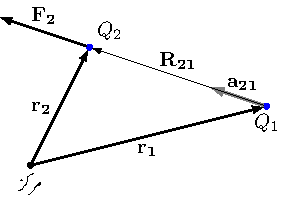
\includegraphics{figCoulombForceBetweenTwoCharges}
\caption{دو مثبت باروں کے مابین قوت دفع}
\label{شکل_سمتیہ_دو_مثبت_بار_قوت_دفع}
\end{figure}
دونوں بار مثبت یا دونوں بار منفی ہونے کی صورت میں \عددیء{Q_2} پر مساوات \حوالہ{مساوات_کولمب_قوت_کی_مساوات_الف} سے قوت \سمتیہ{a_{21}} کی سمت میں حاصل ہوتا ہے۔یوں یکساں باروں کے مابین قوت دفع پایا جاتا ہے۔دو الٹ اقسام کے باروں کی صورت میں \عددیء{Q_2} پر قوت \سمتیہ{-a_{21}} کی سمت میں حاصل ہوتا ہے۔یوں الٹ اقسام کے باروں کے مابین قوت کشش پایا جاتا ہے۔  

\ابتدا{مثال}
شکل \حوالہ{شکل_سمتیہ_دو_مثبت_بار_قوت_دفع} میں نقطہ \عددیء{A(3,2,4)} پر \عددیء{\SI{20}{\micro \coulomb}} کا بار \عددیء{Q_1} جبکہ نقطہ \عددیء{B(1,5,9)} پر \عددیء{\SI{-50}{\micro \coulomb}} کا بار \عددیء{Q_2} پایا جاتا ہے۔منفی بار \عددیء{Q_2} پر سمتی قوت حاصل کریں۔

حل:
\begin{align*}
\kvec{R_{21}}&=(1-3) \ax+(5-2) \ay+(9-4)\az\\
&=-2 \ax+3 \ay+5 \az\\
R_{21}&=\abs{\kvec{R_{21}}}=\sqrt{(-2)^2+3^2+5^2}\\
&=\sqrt{38}\\
&=6.1644
\end{align*}
اور یوں
\begin{align*}
\kvec{a_{21}}&=\frac{{\kvec{R_{21}}}}{\abs{\kvec{R}_{21}}}=\frac{-2 {\ax}+3 {\ay}+5 \az}{6.1644}\\
&=-0.324 \ax+0.487 \ay+0.811\az
\end{align*}
حاصل ہوتا ہے جس سے
\begin{align*}
\kvec{F_2}&=\frac{36 \pi  \times 10^9}{4 \pi} \frac{\left (-50\times 10^{-6} \times 20 \times 10^{-6} \right )}{38} \left(-0.324 \ax+0.487 \ay+0.811\az\right)\\
&=-0.237  \left(-0.324 \ax+0.487 \ay+0.811\az \right) \, \si{\newton}
\end{align*}
حاصل ہوتا ہے۔آپ دیکھ سکتے ہیں کہ قوت کی سمت \سمتیہ{a_{21}} کے الٹ سمت میں ہے۔یوں منفی بار پر قوت کی سمت مثبت بار کی جانب ہے یعنی اس پر قوت کشش پایا جاتا ہے۔
\انتہا{مثال}
%========================
کسی بھی بار پر ایک سے زیادہ باروں سے پیدا مجموعی قوت تمام باروں سے پیدا علیحدہ علیحدہ قوتوں کا سمتی مجموعہ ہوتا ہے یعنی
\begin{align}
\kvec{F}=\sum_{i=1}^n \kvec{F}_i
\end{align}
اس حقیقت کو یوں بیان کیا جاتا ہے کہ کولمب کا قانون \اصطلاح{خطی}\فرہنگ{خطی}\حاشیہب{linear}\فرہنگ{linear} ہے۔ 

%========================
\حصہ{برقی میدان کی شدت}
نیوٹن کے کائناتی تجاذب کے قانون میں زمین کی کمیت کو \عددیء{M} لکھ کر کمیت \عددیء{m} پر قوت \عددیء{F} حاصل کی جا سکتی ہے۔ایک کلوگرام کمیت پر اس قوت کی مقدار \عددیء{\tfrac{F}{m}} ہو گی جسے \اصطلاح{زمین کی کشش}\فرہنگ{کشش!زمین}\حاشیہب{gravity}\فرہنگ{gravity} یا \اصطلاح{ثقلی اسراع} پکارا اور \عددیء{g} لکھا جاتا ہے۔زمین کی سطح پر \عددیء{g} کی مقدار تقریباً \عددیء{\SI{9.8}{\meter \per \second \squared}} کے برابر ہے۔
\begin{align}\label{مساوات_کولمب_زمین_کی_کشش}
g&=\frac{F}{m}=\frac{GM}{R^2}
\end{align}

کسی بھی کمیت \عددیء{M} کے گرد  \اصطلاح{تجاذبی میدان}\حاشیہب{gravitational field}\فرہنگ{تجاذبی میدان} پایا جاتا ہے۔ کسی بھی نقطے پر  اس تجاذبی میدان کو ناپنے کی خاطر اس نقطے پر پیمائشی کمیت \عددیء{m_p}\حاشیہد{\عددیء{m_p} لکھتے ہوئے  زیرنوشت میں \عددیء{p} لفظ پیمائشی  کے \موٹا{پ} کو ظاہر کرتا ہے، یعنی یہ وہ کمیت ہے جسے قوت  کی پیمائش کی خاطر استعمال کیا جا رہا ہے۔} رکھ کر اس پر قوت ناپی جاتی ہے۔مختلف مقامات پر اس طرح قوت ناپ کر ہم تجاذبی میدان کا جائزہ لے سکتے ہیں۔تجاذبی قوت کی مقدار کا دارومدار پیمائشی کمیت \حاشیہب{test mass} \عددیء{m_p} پر بھی منحصر ہے۔مختلف تجاذبی میدانوں کا آپس میں موازنہ کرتے وقت یہ ضروری ہے کہ تمام تجاذبی میدان جانچتے وقت ایک ہی قیمت کے پیمائشی کمیت استعمال کی جائے۔ماہرین طبیعیات عموماً \عددیء{m_p} کو ایک کلوگرام  رکھتے ہیں۔یہ ضروری نہیں کہ تجاذبی قوت ناپتے وقت ایک کلوگرام کی پیمائشی کمیت ہی استعمال کی جائے البتہ جوابات اکٹھے کرتے وقت \سمتیہ{F} کو \عددیء{m_p} سے تقسیم کرتے ہوئے ایک کلوگرام پر تجاذبی قوت حاصل کی جا سکتی ہے۔زمین کے قریب ایک کلو گرام کمیت پر قوت کشش کو ثقلی اسراع \عددی{g} پکارا جاتا ہے۔

\ابتدا{مثال}
زمین کی سطح پر دو سو گرام پیمائشی کمیت پر \عددیء{\SI{1.96}{\newton}} قوت ناپی جاتی ہے۔ثقلی اسراع حاصل کریں۔

حل:
\begin{align}
g=\frac{1.96}{0.2}=\SI{9.8}{\newton \per \kilogram}
\end{align}   
\انتہا{مثال}

مساوات \حوالہ{مساوات_کولمب_زمین_کی_کشش} سے ہم
\begin{gather}
\begin{aligned}
F&=m g\\
w&=m g
\end{aligned}
\end{gather}
لکھ سکتے ہیں جو زمین کی  سطح پر کمیت \عددیء{m} پر کشش ثقل \عددیء{F} دیتا ہے جسے  وزن پکارا اور  \عددیء{w} لکھا جاتا ہے۔
  
باروں پر بھی اسی طرح غور کیا جاتا ہے۔کسی بھی بار \عددیء{Q} کے گرد برقی میدان پایا جاتا ہے یعنی برقی میدان کا منبع بار ہے۔اس برقی میدان میں بار پر قوت اثر انداز ہوتا ہے۔بار \عددیء{Q} کے برقی میدان کی شدت کے پیمائش کی خاطر اس میدان میں مختلف مقامات پر پیمائشی بار \حاشیہب{test charge} \عددیء{q_p} پر قوت \سمتیہ{F} ناپ کر برقی میدان کا مطالعہ کیا جا سکتا ہے اور اس کا نقشہ بنایا جا سکتا ہے۔مختلف باروں کے برقی میدانوں کا آپس میں موازنہ کرتے وقت یہ ضروری ہے کہ تمام صورتوں میں ایک ہی قیمت کے پیمائشی بار  استعمال کئے جائیں۔ماہرین طبیعیات \عددیء{q_p} کو ایک کولمب کا مثبت بار  رکھتے ہیں۔یہ ضروری نہیں کہ قوت ناپتے وقت ایک کولمب کا مثبت پیمائشی بار ہی استعمال کیا جائے البتہ جوابات اکٹھے کرتے وقت \سمتیہ{F} کو \عددیء{q_p} سے تقسیم کرتے ہوئے ایک مثبت کولمب کے بار پر قوت حاصل کی جاتی ہے جسے \اصطلاح{برقی میدان کی شدت}\فرہنگ{برقی میدان!شدت}\فرہنگ{شدت!برقی}\حاشیہب{electric field intensity}\فرہنگ{electric field intensity} یا صرف \اصطلاح{برقی میدان} پکارا اور \سمتیہ{E} لکھا جاتا ہے یعنی
\begin{align}\label{مساوات_کولمب_برقی_شدت_اور_قوت}
\kvec{E}=\frac{\kvec{F}}{q_p}
\end{align}
مختلف مقامات پر موجود مختلف قیمتوں کے باروں سے کسی ایک نقطے پر  پیدا برقی میدان  تمام باروں کے مجموعی اثر سے پیدا ہو گا۔ایسا کولمب کے قانون کے خطی ہونے کی بنا پر ہوتا ہے۔کسی بھی نقطے پر \عددیء{n} باروں کا مجموعی \سمتیہ{E} تمام باروں کے علیحدہ علیحدہ پیدا کردہ  \سمتیازیرنوشت{E}{1}،  \سمتیازیرنوشت{E}{2}،\سمتیازیرنوشت{E}{3}،\عددیء{\cdots}  کا سمتی مجموعہ
\begin{align}
\kvec{E}=\sum_{i=1}^n \kvec{E}_i=\kvecsub{E}{1}+\kvecsub{E}{2}+\kvecsub{E}{3}+\cdots+\kvec{E}_n 
\end{align}
 ہوتا ہے۔یوں کسی بھی نقطے \عددیء{P}  پر \سمتیہ{E} ناپتے وقت اس نقطے پر ایک کولمب بار \عددیء{q_p} رکھ کر اس بار پر قوت ناپی جاتی ہے۔یہ قوت اس نقطے پر تمام باروں کا مجموعی  \سمتیہ{E} ہوتا ہے۔یاد رہے کہ کسی بھی نقطے پر  \سمتیہ{E} ناپتے وقت یہاں رکھے پیمائشی بار \عددیء{q_p} کا اثر شامل نہیں ہوتا۔

مساوات  \حوالہ{مساوات_کولمب_قوت_کی_مساوات_الف} سے  بار \عددیء{Q} سے \عددیء{\kvec{a}_R} سمت میں \عددیء{R} فاصلے پر برقی میدان کو
\begin{gather}
\begin{aligned}\label{مساوات_کولمب_قوت_کی_عمومی_مساوات}
\kvec{E}&=\frac{Q}{4 \pi \epsilon_0}\frac{\kvec{a_{R}}}{ R^2}\\
&=\frac{Q}{4 \pi \epsilon_0}\frac{\kvec{R}}{ R^3}
\end{aligned}
\end{gather}
لکھا جا سکتا ہے۔بار کو کروی محدد کے مرکز پر تصور کرتے ہوئے اسی مساوات کو یوں لکھا جا سکتا ہے
\begin{align}\label{مساوات_کولمب_نقطہ_بار_کروی_رداس_پر_تبدیل_نہیں_ہوتا}
\kvec{E}=\frac{Q}{4 \pi \epsilon_0 r^2} \ar
\end{align}
جہاں  \عددیء{\ar}  کروی محدد کا رداسی سمت میں اکائی سمتیہ ہے۔

نقطہ \عددیء{(x',y',z')} پر موجود بار \عددیء{Q} سے نقطہ \عددیء{(x,y,z)} پر برقی شدت  یوں حاصل کی جا سکتی ہے۔
\begin{gather}
\begin{aligned} \label{مساوات_کولمب_نقطہ_بار_سے_میدان_کا_حصول}
\kvec{E}&=\frac{1}{4 \pi \epsilon_0 }\frac{Q}{\abs{\kvec{r}-\kvec{r'}}^2} \frac{\kvec{r}-\kvec{r'}}{\abs{\kvec{r}-\kvec{r'}}}=\frac{Q}{4 \pi \epsilon_0 }\frac{\kvec{r}-\kvec{r'}}{\abs{\kvec{r}-\kvec{r'}}^3}\\
&=\frac{Q}{4 \pi \epsilon_0}\frac{\left[(x-x')\ax+(y-y')\ay+(z-z')\az\right]}{\left [(x-x')^2+(y-y')^2+(z-z')^2\right]^{\frac{3}{2}}}
\end{aligned}
\end{gather} 
جہاں
\begin{align*}
\kvec{r}&=x \ax+y \ay+z\az\\
\kvec{r'}&=x' \ax+y' \ay+z'\az\\
\kvec{R}&=\kvec{r}-\kvec{r'}=(x-x') \ax+(y-y') \ay+(z-z')\az
\end{align*}
کے برابر ہے۔
%===================
\ابتدا{مثال}
نقطہ \عددیء{N_1(4,1,1)} پر \عددیء{\SI{100}{\micro \coulomb}} کا بار \عددیء{Q_1} جبکہ نقطہ \عددیء{N_2(1,4,2)} پر \عددیء{\SI{50}{\micro \coulomb}} کا بار \عددیء{Q_2} پایا جاتا ہے۔نقطہ \عددیء{N_3(2,2,5)} پر  \عددیء{Q_1} سے پیدا \سمتیازیرنوشت{E}{1}  اور \عددیء{Q_2} سے پیدا \سمتیازیرنوشت{E}{2} حاصل کریں۔اس نقطے پر دونوں باروں کا مجموعی \عددیء{\kvec{E}} کیا ہو گا۔
\begin{figure}
\centering
\includegraphics[height=3.5cm]{figCoulombElectricFieldOfTwoCharges}
\caption{دو باروں سے پیدا برقی شدت}
\label{شکل_کولمب_دو_باروں_سے_پیدا_برقی_شدت}
\end{figure}

حل:شکل \حوالہ{شکل_کولمب_دو_باروں_سے_پیدا_برقی_شدت} میں صورت حال دکھایا گیا ہے۔پہلے \عددیء{Q_1} سے پیدا \سمتیازیرنوشت{E}{1} حاصل کرتے ہیں۔\عددیء{N_1}  سے \عددیء{N_3} تک سمتی فاصلہ
\begin{align*}
\kvecsub{R}{31}=\kvecsub{R}{3}-\kvecsub{R}{1}&=(2-4)\ax+(2-1)\ay+(5-1)\az\\
&=-2\ax+1\ay+4\az
\end{align*}
ہے جس سے
\begin{align*}
R_{31}&=\abs{\kvecsub{R}{31}}=\sqrt{(-2)^2+1^2+4^2}\\
&=\sqrt{21}=4.583\\
\kvecsub{a}{31}&=\frac{\kvecsub{R}{31}}{R_{31}}=\frac{-2\ax+1\ay+4\az}{\sqrt{21}}\\
&=-0.436\ax+0.218\ay+0.873\az
\end{align*}
حاصل ہوتے ہیں۔یوں مساوات \حوالہ{مساوات_کولمب_قوت_کی_عمومی_مساوات} سے
\begin{align*}
\kvecsub{E}{1}&=9 \times 10^9 \frac{100 \times 10^{-6}}{21} \left(-0.436\ax+0.218\ay+0.873\az\right)\\
&=-\num{18686}\ax+\num{9343}\ay+\num{37414}\az \quad \si{\volt \per \meter}
\end{align*}
حاصل ہوتا ہے جہاں مساوات \حوالہ{مساوات_کولمب_برقی_مستقل_قیمت_الف} سے \عددیء{\tfrac{1}{4\pi \epsilon_0}} کی قیمت \عددیء{9 \times 10^9} پر کی گئی۔اسی طرح \عددیء{Q_2} کے لئے حل کرتے ہوئے
\begin{align*}
\kvecsub{R}{32}&=(2-1)\ax+(2-4)\ay+(5-2)\az\\
&=1\ax-2\ay+3\az
\end{align*}
اور
\begin{align*}
R_{32}&=\abs{\kvecsub{R}{32}}=\sqrt{1^2+2^2+3^2}=\sqrt{14}\\
\kvecsub{a}{32}&=\frac{1\ax-2\ay+3\az}{\sqrt{14}}\\
&=0.267\ax-0.535\ay+0.802\az
\end{align*}
سے
\begin{align*}
\kvecsub{E}{2}&=9 \times 10^9 \frac{50 \times 10^{-6}}{14} \left(0.267\ax-0.535\ay+0.802\az \right)\\
&=\num{8582}\ax-\num{17196}\ay+\num{25779}\az \quad \si{\volt \per \meter}
\end{align*}
ملتا ہے۔ان دو جوابات کا سمتی مجموعہ لیتے ہوئے کُل \kvec{E} حاصل کرتے ہیں۔
\begin{align*}
\kvec{E}&=\kvecsub{E}{1}+\kvecsub{E}{2}\\
&=\left(\num{-18686} \ax+\num{9343} \ay+\num{37414}\az\right)+\left(\num{8582}\ax-\num{17196}\ay+\num{25779}\az\right)\\
&=-\num{10104}\ax-\num{7853}\ay+\num{63193}\az \quad \si{\volt \per \meter}
\end{align*} 
\انتہا{مثال}
%===================
 
مساوات \حوالہ{مساوات_کولمب_برقی_شدت_اور_قوت} کو
\begin{align}
\kvec{F}=q \kvec{E}
\end{align}
لکھا جا سکتا ہے جو برقی میدان \سمتیہ{E} کے موجودگی میں بار \عددیء{q} پر قوت \سمتیہ{F} دیتا ہے۔


\حصہ{یکساں بار بردار سیدھی لامحدود لکیر  کا برقی میدان}
شکل \حوالہ{شکل_کولمب_لامحدود_لکیر_پر_بار_کا_میدان} میں \عددیء{z} محدد پر \عددیء{z=-\infty} سے \عددیء{z=+\infty} تک یکساں بار کی کثافت پائی جاتی ہے۔آپ تصور کر سکتے ہیں کہ \عددیء{z} محدد پر انتہائی قریب قریب برابر فاصلے پر یکساں \اصطلاح{نقطہ بار} رکھے گئے ہیں۔یوں اگر \عددیء{\Delta L} لمبائی میں کُل \عددیء{\Delta Q} بار پایا جائے تب اکائی لمبائی میں \عددیء{\tfrac{\Delta Q}{\Delta L}} بار پایا جائے گا جسے \اصطلاح{لکیری کثافتِ بار}\فرہنگ{کثافت!لکیری بار}\حاشیہب{line charge density}\فرہنگ{density!line charge}  \عددیء{\rho_L}\حاشیہد{اس کتاب میں رداس کے لئے بھی \عددیء{\rho} استعمال کیا جاتا ہے۔\عددیء{\rho} کو جب بھی کثافت کے لئے استعمال کیا جائے،اس کے زیر نوشت میں \تحریر{L}، \تحریر{S} یا \تحریر{h} لکھا جائے گا۔} کہا جاتا ہے اور جس کی اکائی \عددیء{\si{\coulomb / \meter}} ہے۔لکیری کثافتِ بار کی تعریف
\begin{align}
\rho_L=\lim_{\Delta L \to 0}\frac{\Delta Q}{\Delta L}
\end{align}
ہے۔لکیر پر چھوٹی لمبائی  اتنی کم نہیں کی جاتی کہ بار بردار الیکٹران علیحدہ علیحدہ نظر آئیں اور لکیری کثافت کی جگہ نقطہ بار نظر آئیں۔اگر لکیر پر بار کی تقسیم ہر جگہ یکساں نہ ہو تب لکیری کثافتِ بار متغیر ہو گی۔آئیں یکساں لکیری کثافتِ بار سے خالی خلاء میں پیدا برقی میدان پر غور کریں۔ 
 \begin{figure}
\centering
\includegraphics[height=3.5cm]{figCoulombElectricFieldOfInfiniteLineCharge}
\caption{یکساں بار بردار سیدھی لامحدود لکیر  کا برقی میدان}
\label{شکل_کولمب_لامحدود_لکیر_پر_بار_کا_میدان}
\end{figure}

پہلے بغیر قلم اٹھائے اس مسئلے کی نوعیت پر توجہ دیتے ہیں۔مقام \عددیء{(0,0,z)} پر  چھوٹی سی لمبائی \عددیء{\Delta z} میں \عددیء{\rho_L \Delta z} بار پایا جاتا ہے جسے نقطہ بار تصور کرتے ہوئے آگے بڑھتے ہیں۔\عددیء{z} محدد کے گرد \عددیء{z=0} یعنی  \عددیء{xy} سطح پر  شکل \حوالہ{شکل_کولمب_لامحدود_لکیر_پر_بار_کا_میدان} میں نقطہ دار گول دائرہ بنایا گیا ہے۔نقطہ بار \عددیء{\rho_L \Delta z} سے دائرے پر کسی بھی مقام پر پیدا برقی میدان پر غور کرتے ہیں۔برقی میدان کی مقدار کا دارومدار میدان پیدا کرنے والے بار اور بار سے فاصلے پر ہے۔نقطہ دار لکیر پر پائے جانے والے تمام نقطوں کا \عددیء{(0,0,z)} سے فاصلہ برابر ہے۔یوں ہم توقع کرتے ہیں کہ اس دائرے پر برقی میدان کی شدت کی حتمی قیمت ہر جگہ برابر ہو گی۔اس کو یوں بھی بیان کیا جا سکتا ہے کہ بار کی نقطہ نظر سے نقطہ دار لکیر پر تمام نقطے بالکل یکساں نظر آتے ہیں۔اس مشابہت سے ہم کہہ سکتے ہیں کہ نقطہ دار دائرے پر ہر جگہ برقی میدان یکساں ہو گا۔ 

آئیں شکل \حوالہ{شکل_کولمب_لامحدود_لکیر_پر_بار_کا_میدان} کو دیکھتے ہوئے  ایک اور مشابہت پر غور کرتے ہیں۔چونکہ \سمتیہ{E} سمتی فاصلہ \سمتیہ{R} کی سمت میں ہوتا ہے لہٰذا دائرے پر کسی بھی نقطے پر نقطہ بار \عددیء{\rho_L \Delta z} سے پیدا  \عددیء{\kvec{E}} کے دو اجزاء پائے جائیں گے یعنی
\begin{align}
\kvec{E}=\kvec{E}_\rho+\kvec{E}_z
\end{align}
مثبت \عددیء{\rho_L} کی صورت میں \عددیء{(0,0,z)} پر موجود بار سے  \عددیء{\kvec{E}_z} کی سمت منفی  \عددیء{z} جانب ہو گی۔اسی طرح \عددیء{(0,0,-z)} پر پائے جانے والے مثبت بار سے دائرے پر پیدا \عددیء{\kvec{E}} کی سمت مثبت \عددیء{z} جانب ہو گی۔دائرے پر یہ دونوں ارکان ایک دونوں کو ختم کریں گے۔اسی عمل سے دائرے پر کسی بھی نقطے پر مثبت \عددیء{z} محدد پر کسی  بھی  فاصلے پر پائے جانے والے بار سے پیدا \عددیء{\kvec{E}_z} کے اثر کو منفی \عددیء{z} محدد پر اتنے ہی فاصلے پر بار سے پیدا  \عددیء{\kvec{E}_z} ختم کرتا ہے۔یوں دائرے پر
\begin{align}\label{مساوات_کولمب_لامحدود_بار_رداس_کا_میدان_صفر}
\kvec{E}_z=0
\end{align}
ہو گا۔

ایک آخری مشابہت پر اب غور کرتے ہیں۔اگر نقطہ دار دائرے کو \عددیء{z} محدد پر مثبت یا منفی جانب  لے جایا جائے تو کیا ہو گا؟ اب بھی دائرے  کے ایک جانب کسی بھی فاصلے پر بار کا اثر دائرے کے دوسری جانب اتنے ہی فاصلے پر بار ختم کرے گا۔یوں دائرے کے ایک جانب یعنی \عددیء{z} محدد پر \عددیء{\infty} تک فاصلے پر باروں کے \عددیء{\kvec{E}_z} کو دائرے کی دوسری جانب \عددیء{z} محدد پر \عددیء{-\infty} تک فاصلے پر باروں کا \عددیء{\kvec{E}_z} ختم کرے گا اور یوں خلاء میں  ہر جگہ مساوات \حوالہ{مساوات_کولمب_لامحدود_بار_رداس_کا_میدان_صفر} درست ثابت ہوتا ہے۔اس حقیقت کو یوں بہتر بیان کیا جا سکتا ہے کہ  لامحدود لکیر پر یکساں کثافت بار  سے خلاء میں برقی میدان صرف رداس کی سمت میں پیدا ہو گا۔آئیں  اس \سمتیہ{E} کو حاصل کریں۔

شکل \حوالہ{شکل_کولمب_لامحدود_لکیر_پر_بار_کا_میدان} میں مقام \عددیء{z} پر نقطہ بار \عددیء{\rho_L \Delta z}  دائرے پر \عددیء{\Delta \kvec{E}} پیدا کرتا ہے۔محدد کے مرکز سے نقطہ بار کا مقام سمتیہ \عددیء{z \az} سے ظاہر کیا جا سکتا ہے جبکہ دائرے پر کسی بھی نقطے \عددیء{N} کو سمتیہ \عددیء{\rho \arho} ظاہر کرتا ہے۔یوں نقطہ بار سے  \عددیء{N} تک کا سمتی فاصلہ اور اسی سمت میں اکائی سمتیہ یوں حاصل کئے جائیں گے۔
\begin{align*}
\kvec{R}&=\rho \arho-z\az\\
\abs{\kvec{R}}&=R=\sqrt{\rho^2+z^2}\\
\kvec{a}_R&=\frac{\kvec{R}}{\abs{\kvec{R}}}=\frac{\rho \arho-z\az}{\sqrt{\rho^2+z^2}}
\end{align*}
مساوات \حوالہ{مساوات_کولمب_نقطہ_بار_کروی_رداس_پر_تبدیل_نہیں_ہوتا} سے
\begin{align*}
\Delta \kvec{E}&=\frac{\rho_L \Delta z}{4 \pi \epsilon_0 \left(\rho^2+z^2 \right)} \frac{\rho \arho-z\az}{\sqrt{\rho^2+z^2}}\\
&=\frac{\rho_L \Delta z \left(\rho \arho-z\az \right)}{4 \pi \epsilon_0\left(\rho^2+z^2 \right)^{\frac{3}{2}}}
\end{align*}
حاصل ہوتا ہے۔تمام باروں کے اثرات کو یکجا کرنے کی خاطر مندرجہ بالا مساوات کو تکمل کی شکل دے کر مندرجہ ذیل مساوات میں دکھایا گیا ہے۔تکملہ کے حدود \عددیء{-\infty} اور \عددیء{+\infty}  ہیں۔
\begin{align}
\kvec{E}=\int \dif  \kvec{E}=\int\limits_{-\infty}^{+\infty} \left[\frac{\rho_L \left(\rho \arho-z\az \right)}{4 \pi \epsilon_0\left(\rho^2+z^2 \right)^{\frac{3}{2}}}\right] \dif z
\end{align}
اس تکمل کو یوں لکھا جا سکتا ہے
\begin{align}\label{مساوات_کولمب_لامحدود_لکیر_بار_کا_میدان}
\kvec{E}&=\frac{\rho_L \rho \arho}{4 \pi \epsilon_0}\int\limits_{-\infty}^{+\infty} \frac{\dif z }{\left(\rho^2+z^2 \right)^{\frac{3}{2}}} -\frac{\rho_L \az}{4 \pi \epsilon_0}\int\limits_{-\infty}^{+\infty} \frac{z \dif z}{\left(\rho^2+z^2 \right)^{\frac{3}{2}}}
\end{align}
جہاں مساوات کی نشان کے دائیں جانب پہلا تکمل  \Erho اور دوسرا تکمل \Ez دیتا ہے  یعنی
\begin{gather}
\begin{aligned}\label{مساوات_کولمب_رداسی_اور_عمودی_برقی_میدان}
\Erho&=\frac{\rho_L \rho \arho}{4 \pi \epsilon_0}\int\limits_{-\infty}^{+\infty} \frac{\dif z }{\left(\rho^2+z^2 \right)^{\frac{3}{2}}}\\
\Ez&=-\frac{\rho_L \az}{4 \pi \epsilon_0}\int\limits_{-\infty}^{+\infty} \frac{z \dif z}{\left(\rho^2+z^2 \right)^{\frac{3}{2}}}
\end{aligned}
\end{gather}

مساوات \حوالہ{مساوات_کولمب_لامحدود_بار_رداس_کا_میدان_صفر} کی مدد سے ہم دیکھ سکتے ہیں کہ دوسرا تکملہ صفر جواب دیگا۔آئیں دونوں تکمل کو باری باری حل کریں۔پہلے \Erho حل کرتے ہیں۔اس مساوات میں
\begin{align*}
z=\rho \tan \alpha
\end{align*}
استعمال کرتے ہیں۔ایسا کرتے ہوئے تکمل کا ابتدائی حد 
\begin{align*}
-\infty &= \rho \tan \alpha_{\textrm{ابتدائی}}\\
\alpha_{\textrm{ابتدائی}} &= -\frac{\pi}{2}
\end{align*}
اور اختتامی حد
\begin{align*}
\infty &= \rho \tan \alpha_{\textrm{اختتامی}}\\
\alpha_{\textrm{اختتامی}} &= \frac{\pi}{2}
\end{align*}
حاصل ہوتے ہیں۔مزید
\begin{align*}
\dif z=\rho \sec^2 \alpha \dif \alpha
\end{align*}
لکھا جائے گا۔یوں
\begin{align*}
\Erho&=\frac{\rho_L \rho \arho}{4 \pi \epsilon_0}\int\limits_{-\frac{\pi}{2}}^{+\frac{\pi}{2}} \frac{\rho \sec^2 \alpha \dif \alpha}{\left(\rho^2+\rho^2 \tan^2 \alpha \right)^{\frac{3}{2}}}\\
&=\frac{\rho_L \rho \arho}{4 \pi \epsilon_0}\int\limits_{-\frac{\pi}{2}}^{+\frac{\pi}{2}} \frac{\rho \sec^2 \alpha \dif \alpha}{\rho^3 \left(1+ \tan^2 \alpha \right)^{\frac{3}{2}}}
\end{align*}
لکھا جائے گا جس میں
\begin{align*}
1+\tan^2 \alpha=\sec^2 \alpha
\end{align*}
استعمال کرتے ہوئے
\begin{gather}
\begin{aligned}\label{مساوات_کولمب_لامحدود_لکیر_رداسی_میدان}
\Erho&=\frac{\rho_L \rho \arho}{4 \pi \epsilon_0}\int\limits_{-\frac{\pi}{2}}^{+\frac{\pi}{2}} \frac{\rho \sec^2 \alpha \dif \alpha}{\rho^3 \sec^3 \alpha}\\
&=\frac{\rho_L  \arho}{4 \pi \epsilon_0 \rho}\int\limits_{-\frac{\pi}{2}}^{+\frac{\pi}{2}} \cos \alpha \dif \alpha\\
&=\frac{\rho_L  \arho}{4 \pi \epsilon_0 \rho} \eval{\sin \alpha}_{-\frac{\pi}{2}}^{\frac{+\pi}{2}}\\
&=\frac{\rho_L }{2 \pi \epsilon_0 \rho} \arho
\end{aligned}
\end{gather}
ملتا ہے جہاں دوسری  قدم پر \عددیء{\sec \alpha=\tfrac{1}{\cos \alpha}} کا استعمال کیا گیا۔

آئیں اب مساوات \حوالہ{مساوات_کولمب_رداسی_اور_عمودی_برقی_میدان} کے   دوسرے جزو کو حل کریں۔اس میں بھی \عددیء{z= \rho \tan \alpha} استعمال کرتے ہیں۔یوں
\begin{align*}
\Ez&=-\frac{\rho_L \az}{4 \pi \epsilon_0}\int\limits_{-\infty}^{+\infty} \frac{z \dif z}{\left(\rho^2+z^2 \right)^{\frac{3}{2}}}\\
&=-\frac{\rho_L \az}{4 \pi \epsilon_0}\int\limits_{-\frac{\pi}{2}}^{+\frac{\pi}{2}} \frac{\rho^2 \tan \alpha  \sec^2 \alpha \dif \alpha}{\left(\rho^2+\rho^2 \tan^2 \alpha \right)^{\frac{3}{2}}}\\
&=-\frac{\rho_L \az}{4 \pi \epsilon_0 \rho}\int\limits_{-\frac{\pi}{2}}^{+\frac{\pi}{2}} \frac{ \tan \alpha  \sec^2 \alpha \dif \alpha}{\left(1+ \tan^2 \alpha \right)^{\frac{3}{2}}}
\end{align*}
سے
\begin{gather}
\begin{aligned}\label{مساوات_کولمب_لامحدود_لکیر_عمودی_میدان}
\Ez&=-\frac{\rho_L \az}{4 \pi \epsilon_0 \rho}\int\limits_{-\frac{\pi}{2}}^{+\frac{\pi}{2}} \frac{ \tan \alpha  \sec^2 \alpha \dif \alpha}{\sec^3 \alpha}\\
&=-\frac{\rho_L \az}{4 \pi \epsilon_0 \rho}\int\limits_{-\frac{\pi}{2}}^{+\frac{\pi}{2}} \sin \alpha \dif \alpha\\
&=\frac{\rho_L \az}{4 \pi \epsilon_0 \rho} \eval{\cos \alpha}_{-\frac{\pi}{2}}^{+\frac{\pi}{2}}\\
&=0
\end{aligned}
\end{gather}
ملتا ہے۔یہی جواب مساوات \حوالہ{مساوات_کولمب_لامحدود_بار_رداس_کا_میدان_صفر} میں حاصل کیا گیا تھا۔

مساوات \حوالہ{مساوات_کولمب_لامحدود_لکیر_رداسی_میدان} اور مساوات \حوالہ{مساوات_کولمب_لامحدود_لکیر_عمودی_میدان} سے مساوات \حوالہ{مساوات_کولمب_لامحدود_لکیر_بار_کا_میدان}  کا حل یوں لکھا جائے گا
\begin{align}\label{مساوات_کولمب_لامحدود_لکیر_رداسی_میدان_پیدا_کرتا_ہے}
\kvec{E}=\Erho=\frac{\rho_L }{2 \pi \epsilon_0 \rho} \arho
\end{align}
جس کے مطابق لامحدود سیدھی لکیر پر یکساں بار سے برقی میدان رداس \عددیء{\rho}  کے بالعکس متناسب ہے۔اس نتیجے  کا مساوات \حوالہ{مساوات_کولمب_نقطہ_بار_کروی_رداس_پر_تبدیل_نہیں_ہوتا} کے ساتھ موازنہ کریں جو نقطہ بار کی برقی میدان بیان کرتا ہے۔نقطہ بار کا برقی میدان کروی رداس کے مربع کے بالعکس متناسب ہے۔یوں اگر لامحدود لکیر کے بار سے فاصلہ دگنا کر دیا جائے تو برقی میدان آدھا ہو جائے گا جبکہ نقطہ بار سے فاصلہ دگنا کرنے سے برقی میدان چار گنا کم ہوتا ہے۔

کسی بھی سمت میں لامحدود سیدھی لکیر پر بار کا برقی میدان مساوات \حوالہ{مساوات_کولمب_لامحدود_لکیر_رداسی_میدان_پیدا_کرتا_ہے} میں بیان خوبیوں پر پورا اترے گا۔ایسی صورت میں کسی بھی نقطے پر \سمتیہ{E} حاصل کرنے کی خاطر اس نقطے سے بار کے لکیر تک کم سے کم فاصلہ \عددیء{R} حاصل کریں۔یہ فاصلہ نقطے سے لکیر پر عمود کھینچنے سے حاصل ہو گا۔اس فاصلے کو \عددیء{\rho} تصور کریں۔لکیر سے عمودی سمت میں نقطے کی جانب اکائی سمتیہ \عددیء{\kvec{a}_R} کو \arho   \, تصور کریں۔ایسی صورت میں مساوات \حوالہ{مساوات_کولمب_لامحدود_لکیر_رداسی_میدان_پیدا_کرتا_ہے} کو
\begin{align}\label{مساوات_کولمب_کسی_ بھی_سمت_میں_لامحدود_لکیر_رداسی_میدان_پیدا_کرتا_ہے}
\kvec{E}=\frac{\rho_L }{2 \pi \epsilon_0 R} \kvec{a}_R
\end{align}
لکھ سکتے ہیں۔
%===================
\ابتدا{مثال}
\عددیء{y} محدد کے  متوازی اور \عددیء{(x,0,0)} سے گزرتی لامحدود لکیر پر \عددیء{\rho_L} کثافت کا بار پایا جاتا ہے۔نقطہ \عددیء{(x',y',z')} پر \سمتیہ{E} حاصل کریں۔شکل \حوالہ{شکل_کولمب_کسی_بھی_سمت_لامحدود_لکیر_پر_بار_کا_میدان} میں صورت حال دکھائی گئی ہے۔
\begin{figure}
\centering
\includegraphics[height=3.5cm]{figCoulombElectricFieldOfInfiniteLineChargeAlongYaxis}
\caption{کسی بھی سمت میں لامحدود لکیر پر بار کی مثال}
\label{شکل_کولمب_کسی_بھی_سمت_لامحدود_لکیر_پر_بار_کا_میدان}
\end{figure}

حل:\عددیء{(x',y',z')} سے بار کے لکیر پر عمود \عددیء{(x,y',0)} پر ٹکراتا ہے۔ان دو نقطوں کا آپس میں فاصلہ \عددیء{\sqrt{(x'-x)^2+z^2}} ہے جبکہ 
\begin{align*}
\kvec{R}&=(x'-x)\ax+z\az\\
\kvec{a}_R&=\frac{(x'-x)\ax+z\az}{\sqrt{(x'-x)^2+z^2}}
\end{align*}
ہیں۔یوں
\begin{align*}
\kvec{E}=\frac{\rho_L}{2 \pi \epsilon_0 \sqrt{(x'-x)^2+z^2}} \kvec{a}_R
\end{align*}
ہو گا۔
\انتہا{مثال}
%================================
\ابتدا{مشق}
\عددیء{y} محدد پر \عددیء{-\infty} سے \عددیء{+\infty} تک \عددیء{\SI{10}{\nano \coulomb \per \meter}} بار کی کثافت پائی جاتی ہے۔ نقطہ \عددیء{N_1(0,0,6)} اور نقطہ  \عددیء{N_2(0,8,6)}  پر \سمتیہ{E} حاصل کریں۔

جواب: دونوں نقطوں پر \عددی{\kvec{E}=30 \az} کے برابر ہے۔
\انتہا{مشق}
%====================

\ابتدا{مشق}
\عددیء{x} محدد پر \عددیء{-\infty} سے \عددیء{+\infty} تک \عددیء{\SI{5}{\nano \coulomb \per \meter}} بار کی کثافت پائی جاتی ہے۔ نقطہ \عددیء{N_1(0,5,0)} اور نقطہ
  \عددیء{N_2(7,3,4)}  پر \سمتیہ{E} حاصل کریں۔

جوابات:\عددیء{\kvec{E}_1=18 \az \, \si{\volt \per \meter}} اور \عددیء{ \kvec{E}_2=18 \left(\frac{3\ay+4\az}{5}\right) \,\si{\volt \per \meter}}

\انتہا{مشق}
%=======================
\حصہ{یکساں بار بردار ہموار لامحدود سطح}
شکل \حوالہ{شکل_کولمب_لامحدود_سطح_پر_بار} میں  \عددیء{z=0} پر لامحدود \عددیء{x-y} سطح دکھائی گئی ہے۔تصور کریں کہ اس پوری  سطح پر انتہائی قریب قریب نقطہ بار یوں رکھے گئے ہیں کہ سطح پر کہیں بھی چھوٹی رقبہ \عددیء{\Delta S} پر  یکساں قیمت کا بار \عددیء{\Delta Q} پایا جاتا ہے۔اس طرح اکائی رقبے پر کل \عددیء{\tfrac{\Delta Q}{\Delta S}} بار پایا جائے گا جسے \اصطلاح{سطحی کثافتِ بار}\فرہنگ{کثافت!سطحی  بار}\حاشیہب{surface charge density}\فرہنگ{density!surface charge} \عددیء{\rho_S} کہتے ہیں۔سطحی کثافتِ بار کی تعریف
\begin{align}\label{مساوات_کولمب_سطحی_کثافت_تعریف}
\rho_S=\lim_{\Delta S \to 0}\frac{\Delta Q}{\Delta S}
\end{align}
ہے۔چھوٹی سطح اتنی کم نہیں لی جاتی کہ اس پر بار بردار الیکٹران علیحدہ علیحدہ بطور نقطہ بار نظر آئیں بلکہ اسے اتنا رکھا جاتا ہے کہ علیحدہ علیحدہ الیکٹران کا اثر قابل نظر انداز ہو۔ سطح پر ہر جگہ بار کا تقسیم یکساں نہ ہونے کی صورت میں \عددیء{\rho_S} کی قیمت متغیر ہو گی۔آئیں لامحدود سطح پر یکساں کثافتِ بار سے خالی خلاء میں  پیدا \سمتیہ{E} حاصل کریں۔

پہلے غور کرتے ہیں کہ آیا مختلف مقامات سے  دیکھتے ہوئے کچھ اخذ کرنا ممکن ہے۔اگر اس بار بردار سطح کے سامنے ہم کھڑے ہو جائیں تو ہمیں سامنے لامحدود بار بردار سطح نظر آئے گی۔سطح سے برابر فاصلے پر ہم جہاں بھی جائیں ہمیں صورت حال میں کوئی تبدیلی نظر نہیں آئے گی۔اسی طرح اگر ہم سطح کی دوسری طرف اتنے ہی فاصلے پر چلے جائیں تو ہمیں صورت حال میں کسی قسم کی کوئی تبدیلی نظر نہیں آئے گی۔اس مشابہت سے ہم کہہ سکتے ہیں کہ ایسی سطح سے برابر فاصلے پر تمام نقطوں  پر یکساں برقی میدان پایا جائے گا۔اس کے برعکس اگر ہم اس سطح سے دور ہو جائیں تو ہمیں سطح قدر دور نظر آئے گی اور ہو سکتا ہے کہ اس تبدیلی سے \سمتیہ{E} پر اثر ہو۔آئیں اب مسئلے کو حساب و کتاب سے حل کرتے ہوئے \سمتیہ{E} حاصل کریں۔
\begin{figure}
\centering
\includegraphics[height=3.5cm]{figCoulombElectricFieldOfInfiniteSurfaceCharge}
\caption{یکساں بار بردار ہموار لامحدود سطح}
\label{شکل_کولمب_لامحدود_سطح_پر_بار}
\end{figure}

شکل \حوالہ{شکل_کولمب_لامحدود_سطح_پر_بار}  میں بار بردار سطح پر  \عددیء{z} محدد کے متوازی دو انتہائی قریب قریب لکیریں کھینچی گئی ہیں جن کے مابین فاصلہ \عددیء{\dif y} ہے۔اس گھیرے گئے رقبے کی چوڑائی \عددیء{\dif y} ہے۔یوں \عددیء{\Delta L} لمبائی اور \عددیء{\dif y} چوڑائی رقبے میں \عددیء{\rho_S \Delta L \dif y} بار پایا جائے گا۔لکیروں سے گھیرے رقبے کو بار کی سیدھی لکیر تصور کیا جا سکتا ہے جس پر اکائی لمبائی کے رقبے پر \عددیء{\tfrac{\rho_S \Delta L \dif y}{\Delta L}} بار پایا جائے گا جسے \عددیء{\rho_L} تصور کیا جا سکتا ہے یعنی
\begin{align}
\rho_L=\rho_S \dif y
\end{align}

لامحدود لکیر پر یکساں بار کی کثافت سے پیدا برقی میدان پر گزشتہ حصے میں غور کیا گیا۔نقطہ \عددیء{(x,0,0)}  پر \سمتیہ{E} حاصل کرتے ہیں۔شکل میں لامحدود بار کی لکیر سے اس نقطے تک کا قریبی سمتی فاصلہ \سمتیہ{R} دکھایا گیا ہے جہاں
\begin{align}
\kvec{R}=x \ax-y\ay
\end{align}
کے برابر ہے جس سے
\begin{gather}
\begin{aligned}
R&=\abs{\kvec{R}}=\sqrt{x^2+y^2}\\
\kvec{a}_R&=\frac{x\ax-y\ay}{\sqrt{x^2+y^2}}
\end{aligned}
\end{gather}
حاصل ہوتے ہیں۔یوں بار بردار لکیر سے \عددیء{(x,0,0)} پر پیدا برقی میدان کو مساوات \حوالہ{مساوات_کولمب_کسی_ بھی_سمت_میں_لامحدود_لکیر_رداسی_میدان_پیدا_کرتا_ہے}  کی مدد سے
\begin{gather}
\begin{aligned}
\dif \kvec{E} &= \frac{\rho_S \dif y}{2 \pi \epsilon_0 \sqrt{x^2+y^2}} \frac{x\ax-y\ay}{\sqrt{x^2+y^2}}\\
&=\frac{\rho_S \dif y \left(x\ax-y\ay \right)}{2 \pi \epsilon_0 \left(x^2+y^2\right)}
\end{aligned}
\end{gather}
لکھا جا سکتا ہے۔اس جواب کو \عددیء{\dif \kvec{E}=\dif \kvec{E}_x+\dif \kvec{E}_y} لکھا جا سکتا ہے جہاں
\begin{gather}\label{مساوات_کولمب_لامحدود_سطح_کی_میدان_کے_اجزاء}
\begin{aligned}
\dif \kvec{E}_x&=\frac{\rho_S x \dif y }{2 \pi \epsilon_0 \left(x^2+y^2\right)}\ax\\
\dif \kvec{E}_y&=-\frac{\rho_S y\dif y }{2 \pi \epsilon_0 \left(x^2+y^2\right)} \ay
\end{aligned}
\end{gather}
کے برابر ہیں۔\عددیء{x} محدد کے ایک جانب بار بردار لکیر مندرجہ بالا برقی میدان پیدا کرتا ہے۔غور کرنے سے معلوم ہوتا ہے کہ \عددیء{x} محدد کے دوسری جانب اتنے ہی فاصلے پر بار بردار لکیر سے پیدا برقی میدان مندرجہ بالا \عددیء{\dif \kvec{E}_y} کو ختم کرے گا۔یوں کسی بھی مثبت \عددیء{y} پر کھینچی لکیر کے \عددیء{\dif \kvec{E}_y}  کو منفی \عددیء{y} پر کھینچی لکیر کا \عددیء{\dif \kvec{E}_y} ختم کرے گا۔\عددیء{x} محدد کے دونوں جانب مسئلے کی مشابہت سے یوں ہم توقع کرتے ہیں کہ
\begin{align}\label{مساوات_کولمب_سطحی_صفر_شدت_حصہ}
\kvec{E}_y=0
\end{align} 
ہو گا۔

آئیں اب حساب و کتاب سے مساوات \حوالہ{مساوات_کولمب_لامحدود_سطح_کی_میدان_کے_اجزاء} کو حل کریں۔پہلے \عددیء{\kvec{E}_x} حاصل کرتے ہیں۔مساوات \حوالہ{مساوات_کولمب_لامحدود_سطح_کی_میدان_کے_اجزاء} میں دئے \عددیء{\dif \kvec{E}_x} کا تکمل لیتے ہیں۔ایسا کرنے کی خاطر
\begin{gather}
\begin{aligned}\label{مساوات_کولمب_مماس_کی_مدد_سے_تکملہ_کا_حصول}
y&=x \tan \alpha\\
\dif y &=x \sec^2 \alpha \dif \alpha
\end{aligned}
\end{gather}
کا استعمال کرتے ہیں۔شکل \حوالہ{شکل_کولمب_لامحدود_سطح_پر_بار} میں \عددیء{\alpha} کی نشاندہی کی گئی ہے۔یوں
\begin{align*}
\kvec{E}_x=\int \dif \kvec{E}_x &=\frac{\rho_S x \ax}{2\pi \epsilon_0}\int_{y=-\infty}^{y=+\infty}\frac{\dif y }{ \left(x^2+y^2\right)}\\
&=\frac{\rho_S x \ax}{2\pi \epsilon_0}\int_{\alpha=-\frac{\pi}{2}}^{\alpha=+\frac{\pi}{2}} \frac{x \sec^2 \alpha \dif \alpha}{x^2\left(1+ \tan^2 \alpha\right)}
\end{align*}
میں \عددیء{\sec^2  \alpha=1+\tan^2 \alpha} کے استعمال سے
\begin{gather}
\begin{aligned}\label{مساوات_کولمب_لامحدود_سطح_عمودی_جزو}
\kvec{E}_x&=\frac{\rho_S\ax}{2\pi \epsilon_0}\int_{\alpha=-\frac{\pi}{2}}^{\alpha=+\frac{\pi}{2}}\dif \alpha\\
&=\frac{\rho_S\ax}{2\pi \epsilon_0} \eval{\alpha}_{-\frac{\pi}{2}}^{+\frac{\pi}{2}}\\
&=\frac{\rho_S}{2 \epsilon_0}\ax
\end{aligned}
\end{gather}
حاصل ہوتا ہے۔آئیں اب \عددیء{\kvec{E}_y} حاصل کریں۔

مساوات \حوالہ{مساوات_کولمب_لامحدود_سطح_کی_میدان_کے_اجزاء} میں دئے \عددیء{\dif \kvec{E}_y} کا تکمل لیتے ہیں۔
\begin{align*}
\kvec{E}_y=\int \dif \kvec{E}_y&=-\frac{\rho_S \ay}{2 \pi \epsilon_0} \int_{y=-\infty}^{y=+\infty}\frac{ y\dif y }{ \left(x^2+y^2\right)}
\end{align*}
تکمل کے نشان کے اندر \عددیء{f(y)=x^2+y^2} لیتے ہوئے  اسے \عددیء{\tfrac{\dif f(y)}{2 f(y)}} لکھا جا سکتا ہے جس کا تکمل \عددیء{\tfrac{\ln f(y)}{2}} ہے۔یوں
\begin{gather}
\begin{aligned}\label{مساوات_کولمب_لامحدود_سطح_افقی_جزو}
\kvec{E}_y&=-\frac{\rho_S \ay}{2 \pi \epsilon_0} \eval{\frac{\ln(x^2+y^2)}{2}}_{y=-\infty}^{y=+\infty}\\
&=0
\end{aligned}
\end{gather}
حاصل ہوتا ہے۔مساوات \حوالہ{مساوات_کولمب_سطحی_صفر_شدت_حصہ} میں یہی جواب حاصل کیا گیا تھا۔

مساوات \حوالہ{مساوات_کولمب_لامحدود_سطح_عمودی_جزو} اور مساوات \حوالہ{مساوات_کولمب_لامحدود_سطح_افقی_جزو} کی مدد سے یکساں بار بردار لامحدود سطح کی برقی میدان
\begin{align}\label{مساوات_کولمب_لامحدود_سطح_کی_برقی-میدان}
\kvec{E}=\frac{\rho_S}{2 \epsilon_0}\kvec{a}_N
\end{align}
لکھی جا سکتی ہے جہاں \عددیء{\kvec{a}_N} اس سطح کا عمودی اکائی سمتیہ ہے۔آپ دیکھ سکتے ہیں کہ سطح سے فاصلہ کم یا زیادہ کرنے سے برقی میدان کی شدت پر کوئی اثر نہیں ہوتا۔سطح کے دونوں جانب برقی میدان اسی مساوات سے حاصل کی جائے گی۔ظاہر ہے کہ سطح کے دونوں جانب کے اکائی عمودی سمتیہ آپس میں الٹ ہیں۔

اب تصور کریں کہ اس سطح کے متوازی \عددیء{x=x_1} پر  ایک اور لامحدود سطح  رکھی جائے جس پر بار کی یکساں کثافت \عددیء{-\rho_S} ہو۔ان دو متوازی سطحوں کو دو دھاتی چادروں سے بنایا گیا \اصطلاح{برق گیر}\فرہنگ{برق گیر}\فرہنگ{کپیسٹر}\حاشیہب{capacitor}\فرہنگ{capacitor} ( کپیسٹر) سمجھا جا سکتا ہے۔کسی بھی نقطے پر کل \سمتیہ{E} دونوں سطحوں پر بار سے پیدا برقی میدان کا مجموعہ ہو گا۔پہلے دونوں سطحوں کے دونوں جانب برقی میدان لکھتے ہیں۔ 
\begin{itemize}
\item
\عددیء{x=0} پر \عددیء{+\rho_S} کثافت کی سطح کا برقی میدان۔
\begin{align*}
\kvec{E}_{x>0}^{+}&=+\frac{\rho_S}{2\epsilon_0} \ax &x>0\\
\kvec{E}_{x<0}^{+}&=-\frac{\rho_S}{2\epsilon_0} \ax &x<0
\end{align*} 
\item
\عددیء{x=x_1} پر \عددیء{-\rho_S} کثافت کی سطح کا برقی میدان۔
\begin{align*}
\kvec{E}_{x>x_1}^{-}&=-\frac{\rho_S}{2\epsilon_0} \ax &x>x_1\\
\kvec{E}_{x<x_1}^{-}&=+\frac{\rho_S}{2\epsilon_0} \ax &x<x_1
\end{align*} 

\end{itemize}
ان نتائج کو استعمال کرتے ہوئے \عددیء{x<0}،\عددیء{x>x_1} اور \عددیء{0<x<x_1} خطوں میں برقی میدان حاصل کرتے ہیں۔
\begin{gather}
\begin{aligned}
\kvec{E}_{x<0}&=\kvec{E}_{x<0}^{+} +\kvec{E}_{x<x_1}^-=-\frac{\rho_S}{2\epsilon_0} \ax+\frac{\rho_S}{2\epsilon_0} \ax =0\\
\kvec{E}_{x>x_1}&=\kvec{E}_{x>0}^{+} +\kvec{E}_{x>x_1}^{-}=+\frac{\rho_S}{2\epsilon_0} \ax-\frac{\rho_S}{2\epsilon_0} \ax=0\\
\kvec{E}_{0<x<x_1}&=\kvec{E}_{x>0}^{+}+\kvec{E}_{x<x_1}^{-}=+\frac{\rho_S}{2\epsilon_0} \ax+\frac{\rho_S}{2\epsilon_0} \ax =\frac{\rho_S}{\epsilon_0} \ax
\end{aligned}
\end{gather}

اس نتیجے کے مطابق دو متوازی لامحدود سطحوں جن پر الٹ یکساں کثافت پائی جائے کے باہر کوئی برقی میدان نہیں پایا جاتا جبکہ سطحوں کے درمیانی خطے میں
\begin{align}\label{مساوات_کولمب_متوازی_چادر_کپیسٹر_کا_میدان}
\kvec{E}=\frac{\rho_S}{\epsilon_0}\ax
\end{align}
برقی میدان پایا جاتا ہے۔اس میدان کی سمت مثبت بار بردار چادر سے منفی بار بردار چادر کی جانب ہوتی ہے۔یہی مساوات ایک ایسے برق گیر (کپیسٹر) کے برقی میدان کے لئے بھی استعمال کیا جا سکتا ہے  جس میں دھاتی چادروں  کی لمبائی اور چوڑائی دونوں چادروں کے درمیانی فاصلے سے کئی گنا زیادہ ہو اور چادروں کے درمیان خالی خلاء یا ہوا پائی جائے۔چادروں کے کناروں کے قریب برق گیر (کپیسٹر) کے اندر اور باہر صورت حال قدر مختلف ہو گی۔ 
%=================================
\ابتدا{مثال}
خلاء میں تین متوازی لامحدود سطح پائے جاتے ہیں جن پر بار کی یکساں کثافت پائی جاتی ہے۔پہلی سطح \عددیء{y=2} پر  \عددیء{\SI{2}{\nano \coulomb / \meter \squared}}، دوسری سطح  \عددیء{y=5} پر  \عددیء{\SI{4}{\nano \coulomb / \meter \squared}} اور تیسری سطح \عددیء{y=10} پر  \عددیء{\SI{-6}{\nano \coulomb / \meter \squared}} کثافت پائی جاتی ہے۔\عددیء{N_1(0,0,0)}، \عددیء{N_2(5,3,4)}،\عددیء{N_3(-2,7,11)} اور \عددیء{N_4(-7,30,22)} پر \سمتیہ{E} حاصل کریں۔

جوابات:\عددیء{0}، \عددیء{144 \pi \ay}، \عددیء{216 \pi \ay} اور  \عددیء{0}
\انتہا{مثال}
%=================================

\حصہ{بار بردار حجم}
ہم نقطہ بار، لامحدود لکیر پر بار اور لامحدود سطح پر بار دیکھ چکے ہیں۔اگلا فطری قدم  بار بردار حجم بنتا ہے لہٰذا اسی پر غور کرتے ہیں۔لکیر اور سطح کے بار  پر غور کرتے ہوئے ہر جگہ یکساں کثافت کی بات کی گئی۔حجم میں بار کی بات کرتے ہوئے اس شرط کو دور کرتے ہوئے کثافت کو متغیرہ تصور کرتے ہیں۔یوں مختلف مقامات پر کثافت کی قیمت مختلف ہو سکتی ہے۔

تصور کریں کہ حجم میں انتہائی قریب قریب نقطہ بار پائے جاتے ہیں۔یوں اگر کسی نقطے پر \عددیء{\Delta h} حجم میں \عددیء{\Delta Q} بار پایا جائے تب اس نقطے پر اوسط حجمی کثافتِ بار \عددیء{\tfrac{\Delta Q}{\Delta h}} ہو گی۔کسی بھی نقطے پر بار کی حجمی  کثافت  یوں بیان کی جاتی ہے۔
\begin{align}
\rho_h=\lim_{\Delta h \to 0} \frac{\Delta Q}{\Delta h}
\end{align} 

کسی بھی حجم میں کل بار   تین درجی تکمل سے حاصل کیا جائے گا۔کارتیسی محدد میں ایسا تکمل یوں لکھا جائے گا۔
\begin{align}
Q=\iiint\limits_{\textrm{h}} \rho_h \dif x \dif y \dif z
\end{align}
جہاں تکمل کے نشان کے نیچے \تحریر{h} حجم کو ظاہر کرتا ہے۔اس طرز کے تکمل کو عموماً ایک درجی تکمل سے ہی ظاہر کیا جاتا ہے یعنی
\begin{align}
Q=\int\limits_{\textrm{h}} \rho_h \dif h
\end{align}


حجم میں \سمتیہ{r'}  نقطے پر چھوٹی سی حجم \عددیء{\Delta h'} میں \عددی{\Delta Q = \rho_h' \Delta h'} بار پایا جائے گا جسے نقطہ بار تصور کیا جا سکتا ہے۔نقطہ \سمتیہ{r} پر اس نقطہ بار کا برقی میدان \عددیء{\dif \kvec{E}} مساوات \حوالہ{مساوات_کولمب_نقطہ_بار_سے_میدان_کا_حصول} سے یوں حاصل ہوتا ہے۔
\begin{align*}
\dif \kvec{E}=\frac{1}{4 \pi \epsilon_0 }\frac{\rho_h' \Delta h'}{\abs{\kvec{r}-\kvec{r'}}^2} \frac{\kvec{r}-\kvec{r'}}{\abs{\kvec{r}-\kvec{r'}}}
\end{align*}
اس مساوات میں  نقطہ \عددیء{r'} پر بار کی کثافت \عددیء{\rho_h'} لکھی گئی ہے۔تمام حجم میں پائے جانے والے بار کا نقطہ \سمتیہ{r} پر میدان مندرجہ بالا مساوات کے تکمل سے یوں حاصل کیا جائے گا۔
\begin{align}\label{مساوات_کولمب_حجم_بار_کا_میدان}
\kvec{E}(\kvec{r})=\frac{1}{4 \pi \epsilon_0 }\int\limits_{\textrm{h}}\frac{\rho_h'  \dif h'}{\abs{\kvec{r}-\kvec{r'}}^2} \frac{\kvec{r}-\kvec{r'}}{\abs{\kvec{r}-\kvec{r'}}}
\end{align}

اس مساوات کی  شکل قدر خوف ناک  ہے البتہ حقیقت میں ایسا ہرگز نہیں۔سمتیہ \سمتیہ{r} اس نقطے کی نشاندہی کرتا ہے جہاں برقی میدان حاصل کرنا درکار ہو۔اس نقطے پر برقی میدان
 کو  \عددیء{\kvec{E}(\kvec{r})} لکھ کر اس حقیقت کی وضاحت کی گئی ہے کہ نقطے کی تبدیلی سے برقی میدان تبدیل ہو سکتا ہے۔کثافت از خود  متغیرہ ہے جس کی قیمت \سمتیہ{r'} پر منحصر ہے۔ \سمتیہ{r'} پر چھوٹی حجم \عددیء{\dif h'} اور بار کی کثافت \عددیء{\rho_h'} لکھے گئے ہیں جہاں \عددیء{'} اس بات کی یاد دہانی کراتا ہے کہ یہ متغیرات نقطہ \عددیء{r'} پر پائے جاتے ہیں۔آخر میں یاد رہے کہ کسی بھی نقطے پر \سمتیہ{E} حاصل کرتے وقت اسی نقطے پر موجود بار کو نظرانداز کیا جاتا ہے۔
%==================================================
\حصہ{مزید مثال}

\ابتدا{مثال}
شکل \حوالہ{شکل_کولمب_محدود_لکیر_پر_بار} میں \عددیء{z=z_1} سے \عددیء{z=z_2} تک کی سیدھی لکیر پر  یکساں \عددیء{\rho_L} پایا جاتا ہے۔نقطہ دار گول دائرے پر \سمتیہ{E} حاصل کریں۔اس گول دائرے کا مرکز  کارتیسی محدد کے مرکز \عددیء{(0,0,0)} پر ہے جبکہ دائرہ از خود \عددیء{z=0} سطح پر پایا جاتا ہے۔ 
\begin{figure}
\begin{subfigure}{0.4\textwidth}
\centering
\includegraphics[height=3.5cm]{figCoulombElectricFieldOfFiniteLineCharge}
\caption{محدود لکیر پر بار کی یکساں کثافت}
\end{subfigure}
%
\begin{subfigure}{0.4\textwidth}
\centering
\includegraphics[height=3.5cm]{figCoulombElectricFieldOfFiniteLineChargeLimits}
\caption{\عددی{z} اور \عددیء{\alpha} کا تعلق}
\end{subfigure}
\caption{محدود لکیر پر بار}
\label{شکل_کولمب_محدود_لکیر_پر_بار}
\end{figure}

حل:شکل \حوالہ{شکل_کولمب_محدود_لکیر_پر_بار} سے واضح ہے کہ نکتہ دار گول دائرے پر \سمتیہ{E} کی حتمی قیمت \عددیء{\abs{\kvec{E}}} یکساں ہو گی۔یوں ہم لکھ سکتے ہیں
\begin{align*}
\kvec{E}&=\frac{\rho_L}{4\pi\epsilon_0} \int_{z_1}^{z_2} \frac{\dif z}{\abs{\rho^2+z^2}} \frac{\rho\arho-z\az}{\sqrt{\rho^2+z^2}}\\
&=\frac{\rho_L \rho\arho}{4\pi\epsilon_0} \int_{z_1}^{z_2} \frac{\dif z}{\abs{\rho^2+z^2}^{\frac{3}{2}}}-\frac{\rho_L \az}{4\pi\epsilon_0} \int_{z_1}^{z_2} \frac{z\dif z}{\abs{\rho^2+z^2}^{\frac{3}{2}}}\\
&=\kvec{E}_\rho +\kvec{E}_z
\end{align*}
دائیں جانب باری باری تکملہ حل کرتے ہیں۔تکملہ حل کرنے کی خاطر \عددیء{z=\rho \tan \alpha} کا تعلق استعمال کرتے ہیں۔\عددیء{\alpha} کا \عددیء{z} کا تعلق شکل \حوالہ{شکل_کولمب_محدود_لکیر_پر_بار}-ب میں دکھایا گیا ہے۔
\begin{align*}
\kvec{E}_\rho&=\frac{\rho_L \rho\arho}{4\pi\epsilon_0} \int_{\alpha_1}^{\alpha_2} \frac{\rho \sec^2 \alpha\dif \alpha}{\abs{\rho^2+\rho^2 \tan^2 \alpha}^{\frac{3}{2}}}\\
&=\frac{\rho_L \arho}{4\pi\epsilon_0 \rho} \eval{\sin \alpha}_{\alpha_1}^{\alpha_2}\\
&=\frac{\rho_L \arho}{4\pi\epsilon_0 \rho} \left(\sin \alpha_2-\sin \alpha_1 \right)
\end{align*}
حاصل ہوتا ہے جہاں
\begin{align*}
\alpha_2&=\tan^{-1} \frac{z_2}{\rho}\\
\alpha_1&=\tan^{-1} \frac{z_1}{\rho}
\end{align*}
کے برابر ہے۔شکل  \حوالہ{شکل_کولمب_محدود_لکیر_پر_بار}-ب سے \عددیء{\sin \alpha=\tfrac{z}{\sqrt{\rho^2+z^2}}} لکھا جا سکتا ہے۔یوں
\begin{align*}
\kvec{E}_{\rho}=\frac{\rho_L \arho}{4\pi\epsilon_0 \rho} \left(\frac{z_2}{\sqrt{\rho^2+z_2^2}}-\frac{z_1}{\sqrt{\rho^2+z_1^2}}\right)
\end{align*}
حاصل ہوتا ہے۔اسی طرح
\begin{align*}
\kvec{E}_z&=-\frac{\rho_L \az}{4\pi\epsilon_0} \int_{z_1}^{z_2} \frac{z\dif z}{\abs{\rho^2+z^2}^{\frac{3}{2}}}\\
&=-\frac{\rho_L \az}{4\pi\epsilon_0} \int_{\alpha_1}^{\alpha_2} \frac{\rho^2 \tan \alpha \sec^2 \alpha \dif \alpha}{\abs{\rho^2+\rho^2 \tan^2 \alpha}^{\frac{3}{2}}}
\end{align*}
سے
\begin{align*}
\kvec{E}_z&=\frac{\rho_L \az}{4\pi\epsilon_0 \rho} \left(\cos \alpha_2 -\cos \alpha_1 \right)\\
&=\frac{\rho_L \az}{4\pi\epsilon_0 } \left(\frac{1}{\sqrt{\rho^2+z_2^2}}-\frac{1}{\sqrt{\rho^2+z_1^2}} \right)
\end{align*}
حاصل ہوتا ہے۔\عددیء{\kvec{E}_{\rho}} اور \عددیء{\kvec{E}_z} کا مجموعہ لیتے ہوئے کل برقی میدان یوں حاصل ہوتا ہے۔
\begin{align}
\kvec{E}=\frac{\rho_L \arho}{4\pi\epsilon_0 \rho} \left(\frac{z_2}{\sqrt{\rho^2+z_2^2}}-\frac{z_1}{\sqrt{\rho^2+z_1^2}}\right)+\frac{\rho_L \az}{4\pi\epsilon_0 } \left(\frac{1}{\sqrt{\rho^2+z_2^2}}-\frac{1}{\sqrt{\rho^2+z_1^2}} \right)
\end{align}

اگر نقطہ دار گول دائرہ \عددی{z=z_0} سطح پر پایا جاتا تب مندرجہ بالا مساوات 
\begin{align*}
\kvec{E}=\frac{\rho_L \arho}{4\pi\epsilon_0 \rho} \left[\frac{z_2-z_0}{\sqrt{\rho^2+(z_2-z_0)^2}}-\frac{z_1-z_0}{\sqrt{\rho^2+(z_1-z_0)^2}}\right]+\frac{\rho_L \az}{4\pi\epsilon_0 } \left[\frac{1}{\sqrt{\rho^2+(z_2-z_0)^2}}-\frac{1}{\sqrt{\rho^2+(z_1-z_0)^2}} \right]
\end{align*}
صورت اختیار کرتا۔
\انتہا{مثال}
%=============================

\ابتدا{مثال}
شکل \حوالہ{شکل_کولمب_گول_دائرے_پر_بار} میں \عددیء{z=0} پر گول دائرہ دکھایا گیا ہے جس پر بار کی یکساں کثافت پائی جاتی ہے۔نقطہ \عددیء{(0,0,z)} پر \سمتیہ{E} حاصل کریں۔

\begin{figure}
\centering
\includegraphics[height=3.5cm]{figCoulombElectricFieldOfCircularLineCharge}
\caption{بار بردار گول دائرہ}
\label{شکل_کولمب_گول_دائرے_پر_بار}
\end{figure}

حل:نلکی محدد استعمال کرتے ہوئے اسے حل کرتے ہیں۔کسی بھی زاویہ پر رداس کھینچتے ہوئے دائرے پر کوئی نقطہ حاصل کیا جا سکتا ہے۔زاویہ میں باریک تبدیلی \عددیء{\Delta \phi} سے لمبائی \عددیء{\rho \Delta \phi} حاصل ہوتی ہے جس پر کل بار \عددیء{\Delta Q=\rho_L \rho \Delta \phi} پایا جائے گا۔یوں بار \عددیء{\Delta Q} مقام \عددیء{\rho \arho} پر پایا جاتا ہے جبکہ \سمتیہ{E} مقام \عددیء{z \az} پر درکار ہے۔آپ دیکھ سکتے ہیں کہ \سمتیہ{E} رداس کی سمت میں ممکن نہیں۔\عددیء{\Delta Q} سے
\begin{align*}
\Delta \kvec{E}=\frac{\rho_L \rho \Delta \phi}{4\pi\epsilon_0 \left(\rho^2+z^2 \right)} \frac{z\az-\rho \arho}{\sqrt{\rho^2+z^2}}
\end{align*}
پیدا ہو گا۔دائرے پر تمام بار کے اثر کے لئے تکملہ لینا ہو گا۔
\begin{align*}
\kvec{E}&=\frac{\rho_L \rho}{4\pi\epsilon_0  \left(\rho^2+z^2 \right)^{\frac{3}{2}}}\int_{0}^{2\pi}(z\az-\rho \arho) \dif \phi
\end{align*}
تکملہ کا متغیرہ \عددیء{\phi} ہے جسے تبدیل کرنے سے \عددیء{\rho} اور \عددیء{z} میں کوئی تبدیلی رونما نہیں ہوتی۔اسی لئے انہیں تکملہ کی نشان سے باہر لے جایا گیا ہے۔حاصل تکملہ کو دو حصوں میں لکھا جا سکتا ہے البتہ معاملہ اتنا سیدھا نہیں جتنا معلوم ہوتا ہے۔\عددیء{\kvec{E}_z} لکھتے ہوئے کارتیسی محدد کی اکائی سمتیہ \سمتیہ{\az} کو تکملہ کے باہر لے جایا جا سکتا ہے چونکہ \عددیء{\phi} کی تبدیلی سے \سمتیہ{\az} تبدیل نہیں ہوتا البتہ  \عددیء{\kvec{E}_{\rho}} لکھتے ہوئے نلکی محدد کی اکائی سمتیہ \عددیء{\arho} کو تکملہ کے باہر نہیں لے جایا جا سکتا چونکہ \عددیء{\phi} کی تبدیلی سے  \عددیء{\arho} کی سمت تبدیل ہوتی ہے۔چونکہ \عددیء{\arho} کی سمت تبدیل ہوتی ہے لہٰذا اس کو مستقل تصور کرنا غلط ہے اور یوں یہ تکملہ کے اندر ہی رہے گا۔ 
\begin{gather}
\begin{aligned}
\kvec{E}_z&=\frac{\rho_L \rho z \az}{4\pi\epsilon_0  \left(\rho^2+z^2 \right)^{\frac{3}{2}}}\int_{0}^{2\pi} \dif \phi\\
\kvec{E}_{\rho}&=-\frac{\rho_L \rho^2}{4\pi\epsilon_0  \left(\rho^2+z^2 \right)^{\frac{3}{2}}}\int_{0}^{2\pi} \arho \dif \phi
\end{aligned}
\end{gather}
پہلے تکملہ کا جواب اب دیکھ کر ہی
\begin{align}
\kvec{E}_z&=\frac{2\pi \rho_L \rho z \az}{4\pi\epsilon_0  \left(\rho^2+z^2 \right)^{\frac{3}{2}}}
\end{align}
لکھا جا سکتا ہے جبکہ دوسرے تکملہ میں \عددیء{\arho=\cos \phi \ax+\sin \phi \ay} لکھتے ہوئے حل کرتے ہیں۔
\begin{align*}
\kvec{E}_{\rho}&=-\frac{\rho_L \rho^2}{4\pi\epsilon_0  \left(\rho^2+z^2 \right)^{\frac{3}{2}}}\int_{0}^{2\pi} (\cos \phi \ax+\sin \phi \ay) \dif \phi\\
&=-\frac{\rho_L \rho^2}{4\pi\epsilon_0  \left(\rho^2+z^2 \right)^{\frac{3}{2}}} \eval{ (\sin \phi \ax-\cos \phi \ay) }_{0}^{2\pi}\\
&=0
\end{align*}

یہی جواب اس طرح بھی حاصل کیا جا سکتا ہے کہ گول دائرے پر تمام بار کو \عددیء{Q=2\pi\rho\rho_L} لکھیں۔یہ بار نقطہ \عددیء{(0,0,z)} سے \عددیء{\sqrt{\rho^2+z^2}} فاصلے پر ہے۔اگر اس تمام بار کو ایک ہی نقطے  \عددیء{(\rho,0,0)} پر موجود تصور کیا جائے تو یہ
\begin{align*}
\kvec{E}_R=\frac{2\pi\rho\rho_L}{4\pi\epsilon_0 \left(\rho^2+z^2 \right)} \kvec{a}_R
\end{align*}
برقی میدان پیدا کرے گا۔بار گول دائرے پر پھیلا ہوا ہے لہٰذا حقیقت میں صرف \عددیء{\az} جانب ہی \kvec{E} پیدا ہوتا ہے۔شکل میں اس تکون کو دیکھتے ہوئے جس کا \عددیء{\kvec{R}} حصہ ہے  آپ دیکھ سکتے ہیں کہ \عددیء{\kvec{E}_R} کا \عددیء{\tfrac{z}{\sqrt{\rho^2+z^2}}} حصہ  حقیقت میں پایا جائے گا۔یوں 
\begin{align*}
\kvec{E}_z=\frac{2\pi\rho\rho_L}{4\pi\epsilon_0 \left(\rho^2+z^2 \right)} \frac{z}{\sqrt{\rho^2+z^2}} \az
\end{align*}
ہی حاصل ہوتا ہے۔

\انتہا{مثال}
%=====================
\ابتدا{مثال}\شناخت{مثال_کولمب_کرہ_بار_کا_میدان}
رداس \عددیء{a} کرہ کی سطح پر یکساں کثافتِ بار \عددیء{\rho_S} پایا جاتا ہے۔کرہ کے باہر اور اس کے اندر برقی میدان \عددیء{\kvec{E}}  حاصل کریں۔کرہ کو کروی محدد کے مرکز پر رکھتے ہوئے حل کریں۔

حل:کرہ کی سطح پر نقطہ \عددیء{M(a,\theta,\phi)} پر چھوٹی رقبہ \عددیء{a^2\sin \theta \dif \theta \dif \phi} میں بار \عددیء{\rho_S a^2 \sin \theta \dif \theta \dif \phi} پایا جائے گا جو  نقطہ \عددیء{N(0,0,b)} پر برقی میدان \عددیء{\dif \kvec{E}} پیدا کرے گا۔محدد کے مرکز سے \عددیء{M} تک سمتی فاصلہ \عددیء{a\ar} جبکہ مرکز سے \عددیء{N} تک سمتی فاصلہ \عددیء{b\az} ہے۔یوں \عددیء{M} سے \عددیء{N} تک سمتی فاصلہ 
\begin{align}
\kvec{R}=b\az-a\ar
\end{align}
لکھا جا سکتا ہے جہاں کارتیسی محدد اور کروی محدد کے اکائی سمتیات استعمال کئے گئے ہیں۔اس طرح
\begin{gather}
\begin{aligned}
\abs{\kvec{R}}=\sqrt{\kvec{R} \cdot \kvec{R}}&= \sqrt{(b\az-a\ar)\cdot (b\az-a\ar)}\\
&=\sqrt{b^2+a^2-2 ab \az \cdot \ar}\\
&=\sqrt{b^2+a^2-2 ab \cos \theta}
\end{aligned}
\end{gather}
اور
\begin{align}
\kvec{a}_R=\frac{\kvec{R}}{\abs{R}}=\frac{b\az-a\ar}{\sqrt{b^2+a^2-2 ab \cos \theta}}
\end{align}
حاصل ہوتے ہیں جہاں صفحہ \حوالہصفحہ{جدول_سمتیہ_کروی_کارتیسی_اکائی_غیر-سمتی_ضرب} پر جدول \حوالہ{جدول_سمتیہ_کروی_کارتیسی_اکائی_غیر-سمتی_ضرب} کے استعمال سے \عددیء{\az \cdot \ar=\cos \theta} لکھا گیا ہے۔

کرہ کی سطح \عددیء{z} محدد کو \عددیء{(0,0,-a)} اور \عددیء{(0,0,a)}  پر چھوتا ہے جہاں  بالترتیب \عددیء{\theta=\pi} اور \عددیء{\theta=0} کے برابر ہیں۔یوں \عددیء{(0,0,-a)} سے \عددیء{N(0,0,b)} تک فاصلہ
\begin{gather}
\begin{aligned}\label{مساوات_کولمب_کرہ_مثبت_محدد}
\sqrt{b^2+a^2-2 ab \cos \pi}&=\sqrt{b^2+a^2+2 ab}\\
&=\sqrt{(b+a)^2}\\
&=b+a
\end{aligned}
\end{gather}
کے برابر ہے جہاں جذر لیتے وقت مثبت جواب چنا گیا ہے چونکہ فاصلہ مقداری\حاشیہد{فاصلہ ہر صورت مثبت ہوتا ہے البتہ سمتی فاصلہ مثبت یا منفی ہو سکتا ہے جہاں سمتی فاصلے کی مقدار مثبت ہی رہتی ہے جبکہ اس کی سمت مثبت یا منفی ہو سکتی ہے۔} ہے جو مثبت قیمت رکھتا ہے۔اسی طرح \عددیء{(0,0,a)} سے \عددیء{N(0,0,b)} تک فاصلہ
\begin{align}\label{مساوات_کولمب_کرہ_مثبت_محدد_الف}
\sqrt{b^2+a^2-2 ab \cos 0}=\sqrt{b^2+a^2-2 ab}
\end{align}
کے برابر ہے۔اگر \عددیء{N} کرہ کے باہر ہو تب \عددیء{b > a} ہو گا اور یہ فاصلہ \عددیء{b-a} کے برابر ہو گا جسے  مساوات \حوالہ{مساوات_کولمب_کرہ_مثبت_محدد_الف} سے یوں
\begin{align}\label{مساوات_کولمب_کرہ_مثبت_محدد_ب}
\sqrt{b^2+a^2-2 ab}&=\sqrt{(b-a)^2}=b-a
\end{align}
حاصل کیا جا سکتا ہے۔اس کے برعکس اگر \عددیء{N} کرہ کے اندر ہو تب \عددیء{a>b} ہو گا اور یہ فاصلہ \عددیء{a-b} کے برابر ہو گا جسے  اور مساوات \حوالہ{مساوات_کولمب_کرہ_مثبت_محدد_الف} سے یوں
\begin{align}\label{مساوات_کولمب_کرہ_مثبت_محدد_پ}
\sqrt{b^2+a^2-2 ab}&=\sqrt{(a-b)^2}=a-b
\end{align}
حاصل کیا جا سکتا ہے۔

اس طرح \عددیء{N} پر
%
\begin{align*}
\dif \kvec{E}= \frac{a^2 \sin \theta \dif \theta \dif \phi}{4 \pi \epsilon_0 R^2} \kvec{a}_R
\end{align*} 
لکھتے ہوئے تمام کرہ پر بار سے پیدا میدان کو تکمل سے یوں حاصل کیا جا سکتا ہے۔
\begin{gather}
\begin{aligned}
\kvec{E}&=\int_{0}^{2\pi} \int_0^{\pi} \frac{\rho_S a^2 \sin \theta \dif \theta \dif \phi}{4 \pi \epsilon_0 (b^2+a^2-2 ab \cos \theta)} \frac{b\az-a\ar}{\sqrt{b^2+a^2-2 ab \cos \theta}}\\
&=\frac{\rho_S a^2}{4 \pi \epsilon_0}\int_{0}^{2\pi} \int_0^{\pi} \frac{ (b\az-a\ar)\sin \theta }{ \left(b^2+a^2-2 ab \cos \theta \right)^{\frac{3}{2}}} \dif \theta \dif \phi
\end{aligned}
\end{gather}
اس مساوات میں جدول \حوالہ{جدول_سمتیہ_کروی_کارتیسی_اکائی_غیر-سمتی_ضرب} کی مدد سے \عددیء{\ar=\sin \theta \cos \phi \ax+\sin \theta \sin \phi \ay+\cos \theta \az} لکھتے ہوئے
\begin{align}\label{مساوات_کولمب_کرہ-سطحی_بار_کثافت_کا_میدان}
\kvec{E}=\frac{\rho_S a^2}{4 \pi \epsilon_0}\int_{0}^{2\pi} \int_0^{\pi} \frac{[-a \sin \theta \cos \phi \ax-a \sin \theta \sin \phi \ay+ (b-a \cos \theta)\az ]\sin \theta }{ \left(b^2+a^2-2 ab \cos \theta \right)^{\frac{3}{2}}} \dif \theta \dif \phi
\end{align}
حاصل ہوتا ہے۔\عددیء{z} محدد سے دیکھتے ہوئے صاف ظاہر ہے کہ اس محدد پر میدان صرف اور صرف \عددیء{\az} سمت میں ہی ممکن ہے۔یوں \عددیء{\ax} اور \عددیء{\ay} اجزاء کو صفر لیتے ہوئے
\begin{align}
E_z=\frac{\rho_S a^2}{4 \pi \epsilon_0}\int_{0}^{2\pi} \int_0^{\pi} \frac{(b-a \cos \theta) \sin \theta }{ \left(b^2+a^2-2 ab \cos \theta \right)^{\frac{3}{2}}} \dif \theta \dif \phi
\end{align}
لکھتے ہیں۔سوال \حوالہ{سوال_کولمب_کرہ_بار_کثافت_کا_میدان_صرف_رداسی_ہے} میں آپ سے  درخواست کی گئی ہے کہ  مساوات \حوالہ{مساوات_کولمب_کرہ-سطحی_بار_کثافت_کا_میدان} میں \عددیء{\ax} اور \عددیء{\ay} اجزاء کو صفر ثابت کریں۔بیرونی تکمل پہلے لیتے ہوئے
\begin{align}
E_z=\frac{2 \pi\rho_S a^2}{4 \pi \epsilon_0} \int_0^{\pi} \frac{(b-a \cos \theta) \sin \theta }{ \left(b^2+a^2-2 ab \cos \theta \right)^{\frac{3}{2}}} \dif \theta
\end{align}
حاصل ہوتا ہے جسے

\begin{align}\label{مساوات_کولمب_کرہ_بار_کا_میدان_الف}
E_z=\frac{2 \pi\rho_S a^2 b}{4 \pi \epsilon_0} \int_0^{\pi} \frac{ \sin \theta \dif \theta}{ \left(b^2+a^2-2 ab \cos \theta \right)^{\frac{3}{2}}}-\frac{2 \pi\rho_S a^3}{4 \pi \epsilon_0} \int_0^{\pi} \frac{\cos \theta \sin \theta \dif \theta}{ \left(b^2+a^2-2 ab \cos \theta \right)^{\frac{3}{2}}}
\end{align}
لکھا جا سکتا ہے۔

مساوات \حوالہ{مساوات_کولمب_کرہ_بار_کا_میدان_الف} کے پہلے تکمل میں \عددیء{w=\cos \theta} اور \عددیء{\dif w=-\sin \theta \dif \theta} پُر کر کے حل کرتے ہوئے
\begin{align}\label{مساوات_کولمب_کرہ_بار_پہلا_تکمل_الف}
\int \frac{ \sin \theta \dif \theta}{ \left(b^2+a^2-2 ab \cos \theta \right)^{\frac{3}{2}}}&=\int \frac{-\dif w}{\left(b^2+a^2-2 ab w \right)^{\frac{3}{2}}}=\frac{-1}{ab (b^2+a^2-2abw)^{\frac{1}{2}}}
\end{align}
یعنی
\begin{align*}
\frac{-1}{ab \sqrt{b^2+a^2-2ab\cos \theta}}
\end{align*}
لکھا جا سکتا ہے۔یوں
\begin{gather}
\begin{aligned}
\int_0^{\pi} \frac{ \sin \theta \dif \theta}{ \left(b^2+a^2-2 ab \cos \theta \right)^{\frac{3}{2}}}&=\left. \frac{-1}{ab \sqrt{b^2+a^2-2ab\cos \theta}} \right|_{0}^{\pi}\\
&=\frac{-1}{ab \sqrt{b^2+a^2+2ab}}+\frac{1}{ab \sqrt{b^2+a^2-2ab}}
\end{aligned}
\end{gather}
حاصل ہوتا ہے جو \عددیء{N} بیرونِ کرہ ہونے کی صورت میں مساوات \حوالہ{مساوات_کولمب_کرہ_مثبت_محدد} اور مساوات \حوالہ{مساوات_کولمب_کرہ_مثبت_محدد_ب} کے تحت
\begin{align}\label{مساوات_کولمب_کرہ_کے_باہر_پہلا_تکمل}
\frac{1}{ab} \left[\frac{-1}{b+a}+\frac{1}{b-a} \right]=\frac{1}{ab} \left[\frac{-(b-a)+(b+a)}{(b+a)(b-a)}\right]=\frac{2}{b(b^2-a^2)}
\end{align}
جبکہ \عددیء{N} اندرونِ کرہ ہونے کی صورت میں مساوات \حوالہ{مساوات_کولمب_کرہ_مثبت_محدد} اور مساوات \حوالہ{مساوات_کولمب_کرہ_مثبت_محدد_پ} کے تحت
\begin{align}\label{مساوات_کولمب_کرہ_کے_اندر_پہلا_تکمل}
\frac{1}{ab} \left[\frac{-1}{a+b}+\frac{1}{a-b} \right]=\frac{1}{ab} \left[\frac{-(a-b)+(a+b)}{(a+b)(a-b)} \right]=\frac{2}{a(a^2-b^2)}
\end{align}
شکل اختیار کرتا ہے۔

مساوات \حوالہ{مساوات_کولمب_کرہ_بار_کا_میدان_الف} کے دوسرے تکمل میں \عددیء{w=\cos \theta} پُر کرتے ہوئے
\begin{align*}
\int \frac{\cos \theta \sin \theta \dif \theta}{ \left(b^2+a^2-2 ab \cos \theta \right)^{\frac{3}{2}}}=\int\frac{-w \dif w}{(b^2+a^2-2abw)^{\frac{3}{2}}}
\end{align*}
حاصل ہوتا ہے۔آپ
\begin{align*}
\int u \dif v = u v-\int v \dif u
\end{align*}
کے کلیہ سے بخوبی واقف ہیں۔ہم
\begin{align*}
u&=w\\
\dif v&=\frac{-\dif w}{(b^2+a^2-2abw)^{\frac{3}{2}}}
\end{align*}
لیتے ہیں۔یوں
\begin{align*}
v=\int \dif v = \int \frac{-\dif w}{(b^2+a^2-2abw)^{\frac{3}{2}}}
\end{align*}
کے برابر ہے جسے ہم مساوات \حوالہ{مساوات_کولمب_کرہ_بار_پہلا_تکمل_الف} میں  حاصل کر چکے ہیں۔اس طرح
\begin{align*}
\int \frac{\cos \theta \sin \theta \dif \theta}{ \left(b^2+a^2-2 ab \cos \theta \right)^{\frac{3}{2}}}&=\int w \left[ \frac{-\dif w}{(b^2+a^2-2abw)^{\frac{3}{2}}} \right]\\
&=w \left[\frac{-1}{ab (b^2+a^2-2abw)^{\frac{1}{2}}}\right]+\int \frac{\dif w}{ab (b^2+a^2-2abw)^{\frac{1}{2}}}\\
&=\frac{-w}{ab (b^2+a^2-2abw)^{\frac{1}{2}}}-\frac{ (b^2+a^2-2abw)^{\frac{1}{2}}}{a^2b^2}\\
&=\frac{-(b^2+a^2-abw)}{a^2b^2(b^2+a^2-2abw)^{\frac{1}{2}}}
\end{align*}
سے
\begin{align*}
\int_0^{\pi} \frac{\cos \theta \sin \theta \dif \theta}{ \left(b^2+a^2-2 ab \cos \theta \right)^{\frac{3}{2}}}&=\left. \frac{-(b^2+a^2-ab\cos \theta)}{a^2b^2(b^2+a^2-2ab \cos \theta)^{\frac{1}{2}}} \right|_0^{\pi}\\
&=\frac{1}{a^2b^2} \left[\frac{-(b^2+a^2+ab)}{\sqrt{b^2+a^2+2ab}} +\frac{(b^2+a^2-ab)}{\sqrt{b^2+a^2-2ab}}\right]
\end{align*}
حاصل ہوتا ہے۔\عددیء{N} کا کرہ سے باہر  ہونے کی صورت میں اس سے
\begin{align}\label{مساوات_کولمب_کرہ_کے_باہر_دوسرا_تکمل}
\frac{1}{a^2b^2} \left[\frac{-(b^2+a^2+ab)}{\sqrt{b^2+a^2+2ab}} +\frac{(b^2+a^2-ab)}{\sqrt{b^2+a^2-2ab}}\right]=\frac{2a}{b^2(b^2-a^2)}
\end{align}
جبکہ \عددیء{N} کا کرہ کے اندر  ہونے کی صورت میں اس سے
\begin{align}\label{مساوات_کولمب_کرہ_کے_اندر_دوسرا_تکمل}
\frac{1}{a^2b^2} \left[\frac{-(b^2+a^2+ab)}{\sqrt{b^2+a^2+2ab}} +\frac{(b^2+a^2-ab)}{\sqrt{b^2+a^2-2ab}}\right]=\frac{2b}{a^2(a^2-b^2)}
\end{align}

حاصل ہوتا ہے۔کرہ کے باہر مساوات \حوالہ{مساوات_کولمب_کرہ_کے_باہر_پہلا_تکمل} اور مساوات \حوالہ{مساوات_کولمب_کرہ_کے_باہر_دوسرا_تکمل}  کو استعمال کرتے ہوئے مساوات \حوالہ{مساوات_کولمب_کرہ_بار_کا_میدان_الف} سے
\begin{gather}
\begin{aligned}\label{مساوات_کولمب_کرہ_بار_کا_میدان_ب}
E_z&=\frac{2 \pi\rho_S a^2 b}{4 \pi \epsilon_0} \left(\frac{2}{b(b^2-a^2)}\right)-\frac{2 \pi\rho_S a^3}{4 \pi \epsilon_0} \left(\frac{2a}{b^2(b^2-a^2)}\right)\\
&=\frac{4 \pi \rho_S a^2}{4\pi \epsilon_0 b^2}\\
&=\frac{Q}{4\pi \epsilon_0 b^2}
\end{aligned}
\end{gather}
حاصل ہوتا ہے جہاں  کرہ پر کُل بار \عددیء{4\pi a^2\rho_S} کو \عددیء{Q} لکھا گیا ہے۔کرہ کے اندر مساوات \حوالہ{مساوات_کولمب_کرہ_کے_اندر_پہلا_تکمل} اور مساوات \حوالہ{مساوات_کولمب_کرہ_کے_اندر_دوسرا_تکمل}  کو استعمال کرتے ہوئے مساوات \حوالہ{مساوات_کولمب_کرہ_بار_کا_میدان_الف}
\begin{gather}
\begin{aligned}\label{مساوات_کولمب_کرہ_بار_کا_میدان_پ}
E_z&=\frac{2 \pi\rho_S a^2 b}{4 \pi \epsilon_0} \left(\frac{2}{a(a^2-b^2)}\right)-\frac{2 \pi\rho_S a^3}{4 \pi \epsilon_0} \left(\frac{2b}{a^2(a^2-b^2)}\right)\\
&=0
\end{aligned}
\end{gather}

مساوات \حوالہ{مساوات_کولمب_کرہ_بار_کا_میدان_ب} بیرون کرہ \عددیء{z} محدد پر میدان دیتا ہے۔چونکہ ہم کسی بھی سمت میں اس محدد کو رکھ سکتے تھے اور میدان اسی محدد کی سمت یعنی رداسی سمت میں ہوتا  لہٰذا یہ ایک عمومی جواب ہے جسے کسی بھی بیرونی نقطے کے لئے
\begin{align}
\kvec{E}=\frac{Q}{4\pi \epsilon_0 r^2} \ar  \quad \quad (r>a)
\end{align}
لکھا جا سکتا ہے۔یہ وہی میدان ہے جو کروی محدد کے مرکز پر \عددیء{Q} نقطہ بار رکھنے سے حاصل ہوتا ہے۔

مساوات \حوالہ{مساوات_کولمب_کرہ_بار_کا_میدان_پ} کے تحت کرہ کے اندر میدان صفر کے برابر ہے۔یہ انتہائی اہم نتیجہ ہے۔ہم کسی بھی مقام کو کرہ یا کسی بھی مکمل بند موصل سطح میں گھیر کر اس مقام پر صفر برقی میدان یقینی بنا سکتے ہیں۔ایسی سطح کو \اصطلاح{فیراڈے پردہ}\فرہنگ{فیراڈے پردہ}\حاشیہب{Faraday shield}\فرہنگ{Faraday shield} کہتے ہیں۔

حصہ \حوالہ{حصہ_گاوس_کروی_بار_بردار_سطح_کا_میدان} میں اسی مسئلے کو انتہائی آسان طریقے سے حل کرنا دکھایا جائے گا۔
\انتہا{مثال}
%=====================

\ابتدا{مثال}
مثال \حوالہ{مثال_کولمب_کرہ_بار_کا_میدان} کے نتائج استعمال کرتے ہوئے  \عددیء{a} رداس کرہ جس میں یکساں \عددیء{\rho_h} حجمی کثافتِ بار پائی جائے کا کرہ کے اندر اور کرہ کے باہر برقی میدان \عددیء{\kvec{E}} حاصل کریں۔

حل:کرہ کے اندر رداس \عددیء{r} پر \عددیء{\dif r} موٹی جھلی کا حجم \عددیء{4 \pi r^2 \dif r} ہو گا جس میں کُل \عددیء{4 \pi \rho_h r^2 \dif r} بار پایا جائے گا۔مثال  \حوالہ{مثال_کولمب_کرہ_بار_کا_میدان} کے مطابق یہ بار \عددیء{r} سے کم رداس کے خطے میں کوئی برقی میدان نہیں پیدا کرتا جبکہ \عددیء{r} سے زیادہ رداس پر یہ میدان پیدا کرے گا۔یوں \عددیء{R} سے کم کسی بھی رداس پر جھلی میں پائے جانے والا بار \عددیء{R} پر میدان پیدا کرے گا جسے
\begin{align}
\kvec{E}=\int_0^{R} \frac{4\pi \rho_h r^2 \dif r}{4\pi \epsilon_0 R^2} \ar=\left. \frac{\rho_h r^3}{3\epsilon_0 R^2} \ar\right|_0^R=\frac{\rho_h R}{3\epsilon_0}\ar \quad \quad (R<a)
\end{align}
لکھ کر حاصل کیا جا سکتا ہے۔بار کرہ کے باہر یعنی \عددیء{R>a} کی صورت میں کرہ میں موجود تمام بار بطور نقطہ بار کردار ادا کرتے ہوئے
\begin{align}
\kvec{E}=\frac{\frac{4}{3} \pi a^3 \rho_h}{4\pi \epsilon_0 R^2}\ar=\frac{ a^3 \rho_h}{3\epsilon_0 R^2}\ar  \quad \quad (R>a)
\end{align}
\انتہا{مثال}
%=======================

\حصہ{برقی میدان کے سمت بہاو خط}\شناخت{حصہ_کولمب_سمت_بہاو_خط}
ہم نے اب تک جتنے بھی مثال دیکھے ان سب میں \عددیء{\kvec{E}} کی شکل سیدھی لکیر کی مانند رہی ہے۔ایسے میدان کا تصوراتی شکل ذہن میں بنانا آسان ہوتا ہے۔یوں نقطہ بار کے میدان کو بار سے ابتدا کرتے ہوئے ہر طرف سمتیوں سے ظاہر کیا جا سکتا ہے۔اب بار کے قریب \عددیء{\kvec{E}} کی قیمت زیادہ اور بار سے دور اس کی قیمت کم ہوتی ہے۔یوں مختلف مقامات پر \عددیء{\kvec{E}} کی لمبائی یہاں کے میدان کی نسبت سے ہو گی۔میدان کو ظاہر کرنے کے دیگر طریقے بھی رائج ہیں۔

آئیں ایسے ہی ایک طریقے پر غور کریں جس میں میدان کو \اصطلاح{سمت بہاو خط} سے ظاہر کیا جاتا ہے۔اس طریقے میں کسی بھی نقطے  پر \عددیء{\kvec{E}} یہاں سے گزرتے سمت بہاو خط کا مماس ہوتا ہے۔جس مقام پر گھنے سمت بہاو خطوط  پائے جائیں ایسے مقام پر \عددیء{\kvec{E}} کی مقدار زیادہ ہوتی ہے اور جہاں ان خطوط کی تعداد کم ہو وہاں میدان کمزور ہوتا ہے۔سمت بہاو خطوط پر تیر کا نشان \عددیء{\kvec{E}} کے مثبت سمت کی نشاندہی کرتا ہے۔
 
کارتیسی محدد میں کسی بھی میدان کو
\begin{align*}
\kvec{E}=E_x\ax+E_y\ay+E_z\az
\end{align*}
لکھا جا سکتا ہے۔یہ مساوات ان میدان کو بھی ظاہر کرتا ہے جو سیدھی لکیر کی مانند نہ ہوں۔آئیں ایسے عمومی میدان پر غور کریں جس میں \عددیء{E_z} کی قیمت صفر کے برابر ہو جبکہ \عددیء{E_x} اور \عددیء{E_y} کی قیمتیں \عددیء{x} اور \عددیء{y} پر منحصر ہو۔کسی بھی نقطہ \عددیء{(x,y)} پر ایسے میدان کو
\begin{align}\label{مساوات_کولمب_عمومی_کارتیسی_میدان}
\kvec{E}=E_x(x,y)\ax+E_y(x,y)\ay
\end{align}
%
\begin{figure}
\centering
\begin{subfigure}{0.4\textwidth}
\centering
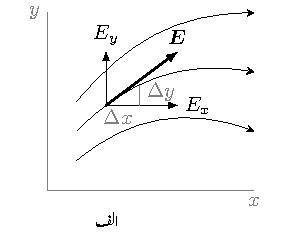
\includegraphics{figCoulombEquipotentials}
\end{subfigure}%
%
\begin{subfigure}{0.4\textwidth}
\centering
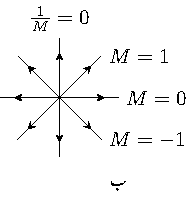
\includegraphics{figCoulombEquipotentialsOfLineCharge}
\end{subfigure}%
\caption{الف) سمت بہاو خط کے مساوات کا حصول۔ ب) لکیری کثافتِ بار کے سمت بہاو خط۔}
\label{شکل_کولمب_سمت_بہاو_خط}
\end{figure}
لکھا  جا سکتا ہے۔شکل \حوالہ{شکل_کولمب_سمت_بہاو_خط}-الف میں ایسے ہی ایک \عددیء{\kvec{E}} کے تین \اصطلاح{سمت بہاو خط} دکھائے گئے ہیں۔شکل میں کسی عمومی نقطے پر \عددیء{\kvec{E}} دکھایا گیا ہے جو اس نقطے سے  گزرتے سمت بہاو خط کا مماس ہے۔میدان کے کارتیسی اجزاء \عددیء{E_x} اور \عددیء{E_y} بھی دکھائے گئے ہیں۔اسی نقطے پر سمت بہاو خط کی چھوٹی لمبائی لیتے ہوئے \عددیء{\Delta x} اور \عددیء{\Delta y} دکھائے گئے ہیں۔\عددیء{\Delta x} اور \عددیء{\Delta y}  کو کم سے کم کرتے ہوئے ہم شکل کو دیکھتے ہوئے
\begin{align}\label{مساوات_کولمب_سمت_بہاو_کارتیسی}
\frac{\dif y}{\dif x}=\frac{E_y}{E_x}
\end{align}
لکھ سکتے ہیں۔اب اگر ہمیں \عددیء{E_x} اور \عددیء{E_y} کی خاصیت معلوم ہو تب ہم تکمل سے سمت بہاو خط کی مساوات حاصل کر سکتے ہیں۔

آئیں لامحدود لکیری کثافتِ بار کے میدان کو مثال بناتے ہوئے اس  کے سمت بہاو خط کی مساوات حاصل کریں۔\عددیء{\rho_L=2\pi \epsilon_0} کی صورت میں \عددیء{z} محدد پر لامحدود لکیری کثافتِ بار کا میدان
\begin{align}\label{مساوات_کولمب_لکیری_میدان_دوبارہ}
\kvec{E}=\frac{\arho}{\rho}
\end{align}
لکھا جاتا ہے۔مساوات \حوالہ{مساوات_کولمب_عمومی_کارتیسی_میدان} بھی اسی میدان کی مساوات ہے جس سے ظاہر ہے کہ \عددیء{E_x=\kvec{E} \cdot \ax} اور \عددیء{E_y=\kvec{E} \cdot \ay} سے حاصل کئے جا سکتے ہیں۔یوں مساوات \حوالہ{مساوات_کولمب_لکیری_میدان_دوبارہ} کی مدد سے
\begin{align*}
E_x&=\frac{1}{\rho} \arho \cdot \ax=\frac{\cos \phi}{\rho}=\frac{x}{x^2+y^2}\\
E_y&=\frac{1}{\rho} \arho \cdot \ay=\frac{\sin \phi}{\rho}=\frac{y}{x^2+y^2}
\end{align*} 
حاصل ہوتے ہیں۔یوں لامحدود لکیری کثافتِ بار کے میدان کو
\begin{align}
\kvec{E}=\frac{x}{x^2+y^2}\ax+\frac{y}{x^2+y^2}\ay
\end{align}
لکھا جا سکتا ہے۔اس طرح مساوات \حوالہ{مساوات_کولمب_سمت_بہاو_کارتیسی} کو
\begin{align*}
\frac{\dif y}{\dif x}=\frac{y}{x}
\end{align*}
یا
\begin{align*}
\frac{\dif y}{y}=\frac{\dif x}{x}
\end{align*}
لکھ کر اس کا تکمل
\begin{align*}
\ln y = \ln x +M'
\end{align*}
یعنی
\begin{align}
y=Mx
\end{align}
لیتے ہوئے میدان کے سمت بہاو خط کی مساوات حاصل کرتے ہیں۔یہ سیدھی لکیر کی مساوات ہے جسے مختلف \عددیء{M} کے قیمتوں کے لئے شکل \حوالہ{شکل_کولمب_سمت_بہاو_خط}-ب میں کھینچا گیا ہے۔

%=====================
\newpage
\حصہء{سوالات}

\ابتدا{سوال}\شناخت{سوال_کولمب_کرہ_بار_کثافت_کا_میدان_صرف_رداسی_ہے}
صفحہ \حوالہصفحہ{مساوات_کولمب_کرہ-سطحی_بار_کثافت_کا_میدان} پر مساوات \حوالہ{مساوات_کولمب_کرہ-سطحی_بار_کثافت_کا_میدان} میں \عددیء{\ax} اور \عددیء{\ay} اجزاء کا تکمل لیتے ہوئے انہیں صفر کے برابر ثابت کریں۔
\انتہا{سوال}
%=========================

\ابتدا{سوال}
تکون کے تینوں کونوں پر \عددی{\SI{25}{\micro\coulomb}} کا بار پایا جاتا ہے جبکہ تینوں کونوں سے \عددیء{\SI{15}{\centi\meter}} فاصلے پر \عددی{\SI{20}{\micro\coulomb}} بار پایا جاتا ہے۔تکون کے اطراف \عددی{\SI{10}{\centi\meter}} ہونے کی صورت میں چوتھے بار پر قوت دفع  کی مقدار حاصل کریں۔

 جواب:\عددی{\SI{0.553}{\newton}}
\انتہا{سوال}
%=====================
\ابتدا{سوال}
\عددی{z=0} پر \عددی{\SI{4}{\nano\farad}} اور \عددی{z=\SI{1}{\centi\meter}} پر \عددی{\SI{-3}{\nano\farad}} بار پائے جاتے ہیں۔\عددی{z} محدد پر وہ نقطے دریافت کریں جہاں مثبت بار پر صفر قوت پائی جائے گی۔

جوابات: \عددی{z=\SI{0.92}{\centi\meter}}، \عددی{z=\SI{7.08}{\centi\meter}}
\انتہا{سوال}
%====================
\ابتدا{سوال}
ایک چکور کے اطراف \عددی{\SI{25}{\centi\meter}} ہیں جبکہ اس کے چاروں کونوں پر \عددی{\SI{30}{\nano\coulomb}} بار پایا جاتا ہے۔کسی ایک کونے کے بار پر کتنی قوت عمل کرے گی۔

جواب:\عددی{\SI{0.248}{\milli \newton}}
\انتہا{سوال}
%===================
\ابتدا{سوال}
نقطہ \عددی{(2,1,-3)} پر \عددی{\SI{15}{\nano\coulomb}} اور نقطہ \عددی{(-3,-5,4)} پر \عددی{\SI{-6}{\nano\coulomb}} بار پایا جاتا ہے۔نقطہ \عددی{(2,1,-3)} پر برقی شدت \عددی{\kvec{E}} حاصل کریں۔

جواب:\عددی{ -0.191\ax+1.057\ay+2.195\az}
\انتہا{سوال}
%===================
\ابتدا{سوال}
نقطہ \عددی{(0,0,3)} اور \عددی{(0,0,-3)} پر \عددی{\SI{20}{\micro\coulomb}} بار پائے جاتے ہیں۔نقطہ \عددی{N(2,0,0)} پر برقی شدت \عددی{\kvec{E}} حاصل کریں۔محدد کے مرکز پر کتنا بار نقطہ \عددی{N} پر اتنی ہی برقی شدت پیدا کرے گا۔

جوابات:\عددی{\kvec{E}=\num{15339}\ax \, \si{\volt\per\meter}}، \عددی{\SI{6.827}{\micro\coulomb}}
\انتہا{سوال}
%===============
\ابتدا{سوال}
نقطہ \عددی{(4,-2,7)} پر \عددی{\SI{5}{\micro\coulomb}} اور \عددی{(-3,4,-2)} پر \عددی{\SI{12}{\micro\coulomb}} بار پایا جاتا ہے۔\عددی{y} محدد پر کہاں \عددی{E_x=0} ہو گا۔

جواب:\عددی{y=-6.89}، \عددی{y=-22.11}
\انتہا{سوال}
%==============
\ابتدا{سوال}
نقطہ \عددی{P(6,3,7)} پر \عددی{\SI{6}{\micro\coulomb}} پایا جاتا ہے۔نقطہ \عددی{N(5,4,2)} پر کارتیسی، نلکی اور کروی  محدد میں \عددی{\kvec{E}} حاصل کریں۔نقطہ \عددی{N} کے اکائی سمتیات استعمال کریں۔
-
جوابات:\عددی{\kvec{E}=-384.4\ax+384.4\ay-1922\az}، \عددی{\kvec{E}=-60\arho+540\aphi-1922\az}، \\
\عددی{\kvec{E}=-630\ar+1817\atheta+540\aphi}
\انتہا{سوال}
%====================
\ابتدا{سوال}
نقطہ \عددی{(0,0,0.25)} اور \عددی{(0,0,-0.25)} پر \عددی{\SI{50}{\nano\coulomb}} جبکہ \عددی{(0,0,0)} پر \عددی{\SI{-35}{\nano\coulomb}} پایا جاتا ہے۔نقطہ \عددی{N(3,1,2)} پر کارتیسی اور کروی محدد میں \عددی{\kvec{E}} حاصل کریں۔

جواب:\عددی{34\ax+11\ay+22\az} ، \عددی{42\ar+0.39\atheta}
\انتہا{سوال}
%===================
\ابتدا{سوال}
محدد کے مرکز پر \عددی{\SI{1}{\nano\coulomb}} بار پایا جاتا ہے۔ سطح \عددی{z=0} پر اس خط کی مساوات حاصل کریں جس پر \عددی{E_y=\SI{1}{\volt\per\meter}} ہو گا۔

جواب:\عددی{80.8y^2=(x^2+y^2)^3}، \عددی{\rho^2=8.987\sin\phi}
\انتہا{سوال}
%====================
\ابتدا{سوال}
محدد کے مرکز پر پڑے چکور کے چاروں کونوں پر \عددی{\SI{5}{\nano\coulomb}} نقطہ بار پائے جاتے ہیں۔چکور \عددی{z=0} سطح پر پایا جاتا ہے جبکہ اس کے اطراف \عددی{\SI{1}{\meter}} لمبے ہیں۔نقطہ \عددی{(0,a,0)} اور نقطہ \عددی{(0,2a,0)} پر برقی شدت کی شرح \عددی{a=2}، \عددی{a=10} اور \عددی{a=\infty} کی صورت میں حاصل کریں۔

جوابات:\عددی{4.15}، \عددی{4.01}، \عددی{4}
\انتہا{سوال}
%===================================
\ابتدا{سوال}
نقطہ \عددی{(0,0,0)} پر \عددی{Q_1} اور نقطہ \عددی{(1,0,0)} پر \عددی{Q_2} نقطہ بار پائے جاتے ہیں۔نقطہ \عددی{(2,1,0)} پر \عددی{E_x=0} ہونے کی صورت میں باروں کا تعلق دریافت کریں۔ 

جواب:\عددی{Q_1=-1.976Q_2}
\انتہا{سوال}
%===============================
\ابتدا{سوال}
کارتیسی محدد کے پہلے آٹھویں حصے \عددی{(x>0,y>0,z>0)} میں حجمی کثافت بار \عددی{\rho_h=10e^{-2z}(x^2+2y^2)} ہے جبکہ بقایا سات حصوں میں کوئی بار نہیں پایا جاتا۔خطہ \عددی{(0\le x\le1,\, 0\le y\le1, \,0\le z\le1)} میں کل بار حاصل کریں۔اسی طرح خطہ \عددی{{(0\le x+2y\le1, \, 0 \le z\le1)}} میں کل بار حاصل کریں۔

جوابات:پہلا جواب \عددی{\SI{4.32}{\coulomb}} ہے۔دوسرا تکمل \عددی{\int_{0}^{1\!/\!2}\int_{0}^{1-2y}\int_{0}^{1}\rho_h \dif z \dif x \dif y} لکھتے ہوئے \عددی{\SI{0.27}{\coulomb}} حاصل ہو گا۔ 
\انتہا{سوال}
%============================
\ابتدا{سوال}
حجمی کثافت بار \عددی{\rho_h=(\rho+0.002)z^2\tan\phi \, \si{\coulomb \per \meter^3}} خطہ \عددیء{0\le \rho \le 0.008}، \عددی{30^{\circ} \le \phi \le 75^{\circ}}، \عددیء{2 \le z \le 5} میں پایا جاتا ہے۔ کثافت بار کی زیادہ سے زیادہ قیمت دریافت کریں۔اس خطے میں کل بار حاصل کریں۔

جوابات:\عددی{\SI{0.933}{\coulomb\per\meter^3}}، \عددی{\SI{11.05}{\micro\coulomb}}
\انتہا{سوال}
%====================
\ابتدا{سوال}
نلکی محدد میں \عددی{z} محدد کے گرد یکساں حجمی کثافت بار \عددیء{e^{-\rho^2}} پائی جاتی ہے۔\عددی{z=0} تا \عددی{z=1} کل بار حاصل کریں۔\عددی{z} محدد کے گرد کتنے رداس کے اندر کل بار کا آدھا پایا جاتا ہے۔

جوابات:\عددی{\SI{3.142}{\coulomb}}، \عددی{\SI{0.832}{\meter}} 
\انتہا{سوال}
%=================
\ابتدا{سوال}
کروی محدد میں رداس کے ساتھ بدلتی حجمی کثافت بار \عددی{\rho_h=\sqrt{r}} پائی جاتی ہے۔اکائی رداس کے کرہ میں کل بار حاصل کریں۔اسی طرح خطہ \عددی{{(r \le 0.5, \theta \le 25^{\circ}, \phi \le \tfrac{\pi}{3})}} میں کل بار حاصل کریں۔ 

جوابات:\عددی{\SI{3.59}{\coulomb}}، \عددی{\SI{0.028}{\coulomb}}
\انتہا{سوال}
%=================
\ابتدا{سوال}
\عددی{x} محدد پر \عددی{\rho_L=\SI{5}{\nano\coulomb\per\meter}} لکیری کثافت بار پایا جاتا ہے جبکہ نقطہ \عددی{(0,3,0)} پر \عددی{\SI{-2}{\nano\coulomb}} نقطہ بار پایا جاتا ہے۔نقطہ \عددی{(4,8,1)} پر \عددی{\kvec{E}} حاصل کریں۔

 

جواب:\عددی{-0.26\ax+10.73\ay+1.32\az \, \si{\volt\per\meter}}
\انتہا{سوال}
%==========================
\ابتدا{سوال}
نقطہ \عددی{(0,2,0)} اور \عددی{(0,0,4)} سے گزرتی سیدھی لکیر پر لکیری کثافت بار \عددی{\SI{2}{\nano\coulomb\per\meter}} پایا جاتا ہے جبکہ نقطہ \عددی{(6,1,-2)} پر \عددی{\SI{7}{\nano\coulomb}} بار پایا جاتا ہے۔نقطہ \عددی{(6,8,4)} پر \عددی{\kvec{E}} حاصل کریں۔

جواب:\عددی{2.47\ax+3.78\ay+1.65\az \, \si{\volt\per\meter}}
\انتہا{سوال}
%===============
\ابتدا{سوال}
کارتیسی \عددی{z} محدد کے کچھ حصہ \عددی{0\le z} پر لکیری کثافت بار \عددی{\SI{5}{\micro\coulomb\per\meter}} پایا جاتا ہے۔نقطہ  \عددی{(0,0,-2)} اور نقطہ  \عددی{(5,-2,6)} پر برقی شدت \عددی{\kvec{E}} حاصل کریں۔

جوابات:\عددی{-22.5\az \, \si{\volt \per\meter}}، \عددی{13.5\ax+5.4\ay-5.5\az\,\si{\volt\per\meter}}
\انتہا{سوال}
%==============================
\ابتدا{سوال}
کارتیسی \عددی{z} محدد کے کچھ حصہ \عددی{2\le z \le 10} پر لکیری کثافت بار \عددی{\SI{2}{\micro\coulomb\per\meter}} پایا جاتا
 ہے۔نقطہ \عددی{(2,12,8)} پر برقی شدت \عددی{\kvec{E}} حاصل کریں۔

\عددی{147\ax+881\ay+133\az \, \si{\volt\per\meter}}
\انتہا{سوال}
%=================================
\ابتدا{سوال}
سطح \عددی{y=1} پر \عددی{\rho_S=\SI{0.72}{\nano\coulomb\per\meter\squared}}، سطح \عددی{y=-3} پر \عددی{\rho_S=\SI{-0.72}{\nano\coulomb\per\meter\squared}}، سطح \عددی{x=-6} پر \عددی{\SI{0.4}{\nano\coulomb\per\meter\squared}} اور لکیر \عددی{x=2,\, z=3} پر
 \عددی{0.4\pi\, \si{\nano \coulomb\per\meter}} پایا جاتا ہے۔نقطہ \عددی{(1,3,-1)} پر \عددی{\kvec{E}} حاصل کریں۔

جواب:\عددی{21.3\ax-5.31\az \,\si{\volt\per\meter}}
\انتہا{سوال}
%=================================
\ابتدا{سوال}
سطح \عددی{z=0} پر مستطیل خطہ \عددی{-2\le x\le 2, \, -3 \le y \le 3}  پر \عددی{\rho_S=\abs{x}\/ \si{\nano\coulomb\per\meter\squared}} پایا جاتا ہے۔نقطہ \عددی{(0,0,3)} پر برقی میدان \عددی{\kvec{E}} حاصل کریں۔

جواب:\عددی{\SI{13.36}{\volt\per\meter}}
\انتہا{سوال}
%================================
\ابتدا{سوال}
سطح \عددی{z=0} پر نلکی رداس \عددی{\rho=2} تا \عددی{\rho=5} سطحی کثافت بار \عددی{\rho_S=\SI{4}{\nano\coulomb\per\meter\squared}} پایا جاتا ہے۔نقطہ \عددی{(0,0,5)} پر برقی شدت \عددی{\kvec{E}} حاصل کریں۔

جواب:\عددی{\SI{50}{\volt\per\meter}}
\انتہا{سوال}
%===================================
\ابتدا{سوال}
میدان \عددی{\kvec{E}=3\sqrt{x}y\ax+x^3y^2\ay} کا سمت بہاو خط حاصل کریں۔نقطہ \عددی{(4,1,7)} پر میدان کی سمت میں اکائی سمتیہ لکھیں۔

جوابات:\عددی{\tfrac{y^2}{2}=\tfrac{x^{3.5}}{3.5}+C}، \عددی{ 0.093\ax+0.996\ay}
\انتہا{سوال}
%=======================
\ابتدا{سوال}
میدان \عددی{\kvec{E}=(x+2)\ax+(4-y)\ay} کے اس سمت بہاو خط کی مساوات حاصل کریں جو نقطہ \عددی{(5,7,2)} سے گزرتی ہے۔

جواب:\عددی{(y-4)(x+2)=21}
\انتہا{سوال}
%====================
\ابتدا{سوال}
جو میدان \عددی{z} تبدیل کرنے سے تبدیل نہیں ہوتے، نلکی محدد میں ان کی سمت بہاو خط \عددی{\tfrac{\dif \rho}{\rho \dif \phi}=\tfrac{E_{\rho}}{E_{\phi}}} حل کرتے ہوئے حاصل کئے جاتے ہیں۔نقطہ \عددی{(5,75^{\circ},3)} سے گزرتے  میدان \عددی{\kvec{E}=\rho\cos\phi\arho+\sin\phi\aphi} کی سمت بہاو خط حاصل کریں۔

جواب:\عددی{\tfrac{1}{\rho}+\ln (\sin \phi)=0.1653}
\انتہا{سوال}
%=======================
